\chapter{Einleitung}

„Es gibt keine Norm für das Menschsein. Es ist normal, verschieden zu sein“ (Weizsäcker 1993).
 

Dieses aus einer Ansprache des ehemaligen Bundespräsidenten entnommene Zitat spiegelt den Leitgedanken von Inklusion wider, demnach alle Menschen mit augenscheinlichen Besonderheiten, jene mit befremdlichen Verhaltensweisen, mit Behinderungen, jene, mit denen die Kommunikation erschwert erscheint oder die in Armut leben, in die Gemeinschaft aufgenommen und von dieser bejaht werden sollen. 
Was aber diese 'schöne Idee', dass alle dazugehören und sich auch dazugehörig fühlen, konkret bedeutet und welche Konsequenzen sich daraus für die pädagogische Praxis ergeben, soll in dieser Arbeit hinterfragt werden.

Inklusion ist ein zentrales Anliegen der heutigen Zeit und eine sozial-ethische, eine politische und eine pädagogische Frage von gesamtgesellschaftlicher Bedeutung. Verstärkt in den Fokus öffentlicher Debatten ist Inklusion durch die Ratifizierung der UN-Behindertenrechtskonvention gerückt.
Um das Thema im Rahmen dieser Bachelorthesis bearbeiten zu können, wird 
sich die Inklusionsfrage auf den Elementarbereich, konkret auf den Kindergarten, beziehen. Verschiedene Autoren weisen auf das große Potential hin, das mit der Umsetzung von Inklusion im Kindergarten verbunden ist, da dort noch keine vereinheitlichten Leistungen wie in der Schule erwartet werden, der Leistungs- und Konkurrenzdruck nicht im Vordergrund steht und weniger starke Exklusionsmechanismen wirken. Zudem wird inklusive Erziehungs- und Bildungsarbeit als wertvolles Ziel betrachtet, weil durch frühe Sozialisation, wenn Heterogenität bereits im Kindergarten gelernt und als positiv erlebt wird, ein gemeinsames Zusammenleben aller als normal erfahren werden kann und das wiederum die Voraussetzung für ein neues gesellschaftliches Bewusstsein darstellt. Auch verbindet sich mit der Bereitstellung einer bestmöglichen Entwicklungsumgebung für alle Kinder die bildungspolitische Hoffnung, dass herkunftsbedingte Benachteiligung in Familien aus Armutslagen kompensiert werden können (vgl. Kron, Papke, Windisch 2010, Albers 2011, Jerg 2011). 

Der Begriff der Inklusion löst den der Integration ab. Mit dem Begriff der Integration wird nach Görannson (2010, 20) oftmals nicht mehr als die organisatorische Maßnahme der Platzierung des Kindes mit Behinderung in einer Gruppe mit Kindern ohne Behinderung verbunden. Inklusion fordert hingegen mehr als die Anpassung des Individuums an das bereits bestehende System, nämlich laut Köhler (2009, 7) radikale Toleranz und den Verzicht auf die Enteignung individueller Lebensschicksale mit Verweis auf eine abstrakte Durchschnittsnorm. Eine erste Annäherung an den Begriff der Inklusion kann sich auf Kron (2010, 15 f.) beziehen. Sie definiert selbigen als Prozess, als kontinuierliches Bemühen, das darauf abzielt, ein angemessenes Umfeld für ’alle’ Kinder zu schaffen. Das hat Konsequenzen für die pädagogische Arbeit und bedeutet somit, dass alle Konzepte, Aktivitäten und Interaktionen an die unterschiedlichen Bedürfnisse, Interessen und Potentiale der Kinder anzupassen sind und gemeinsam mit ihnen, den Eltern und Fachkräften erarbeitet werden, nicht umgekehrt, wie bei der Zuweisung eines Integrationsplatzes häufig geschehen, dass sich die Kinder mit erhöhtem Unterstützungsbedarf den im Vorfeld von ihnen unabhängig entworfenen Vorstellungen anzupassen haben.  

Obwohl Statistiken der Kinder- und Jugendhilfe zu Tageseinrichtungen zeigen, dass etwa 75~\% der Kinder mit erhöhtem Unterstützungsbedarf in Einrichtungen mit inklusiven Werten betreut werden und somit laut Sarimski (2011, 4) die gemeinsame Erziehung und Bildung von Kindern mit und ohne Entwicklungserschwernisse mit großem Abstand am weitesten in den Einrichtungen des Elementarbereiches umgesetzt ist, muss festgehalten werden, dass die deutsche Bildungslandschaft bezüglich der Umsetzung inklusiver Werte in ihrer zuvor aufgezeigten Tragweite noch ganz am Anfang steht. Im Hinblick auf die aktuellen Forschungsergebnisse ergibt sich ein ähnliches Bild. Laut Göransson (2010, 21) besteht die Herausforderung der Forschung darin einen Beitrag zur Entwicklung einer inklusiven Bildung und Erziehung zu leisten. Der Beitrag, der im Rahmen dieser Bachelorthesis geleistet wird, ist unter die Forschungsfrage gestellt: Unter Berücksichtigung welcher Aspekte ist Inklusion im Kindergarten umsetzbar?

\paragraph{Gang durch die Arbeit (unvollständig)} 
Die vorliegende Arbeit ist in einen Teil I und einen Teil II gegliedert. Der Teil I umfasst die theoretischen und konzeptionellen Hintergründe inklusiver Erziehungs- und Bildungsarbeit im Kindergarten und umfasst die Kapitel 2 bis 4. Teil II unter Kapitel 5 beschreibt die empirische Studie, gefolgt von einer Zusammenfassung und Interpretation der Ergebnisse dieser in Kapitel 6. Dem schließt sich eine Schlussbetrachtung und ein Ausblick in Kapitel 7 an sowie zuletzt das Literaturverzeichnis und der Anhang.

Da der Bezugsrahmen für die Umsetzung von Inklusion der Kindergarten ist, wird zuerst der Kindergarten als Erziehungs- und Bildungseinrichtung vorgestellt, erste Verweise auf Aspekte inklusiver Erziehung und Bildung werden hier bereits aufgegriffen.  
Zuvorderst wird die Entwicklung des Kindergartens von der Betreuungs- zur Bildungseinrichtung nachgezeichnet, um das Subsystem Kindergarten in Bezug zu dem Gesellschaftssystem zu stellen (Kapitel 2.1). Daran schließt sich die Darstellung der gesetzlich bindenden Grundlagen an, da bei der Frage nach der bestmöglichen Umsetzung von Inklusion im Kindergarten Richtlinien und geltende Bildungsempfehlungen der Bildungspläne im Auge behalten werden müssen (Kapitel 2.2).    
Im Folgenden (Kapitel 2.3) wird die Diskussion über das Selbstverständnis des Kindergartens fortgesetzt.
Da Inklusion nur unter der Wahrung von Qualitätsstandards umzusetzen ist, werden die für den Bereich der pädagogischen Qualität geltenden Qualitätsdimensionen aufgezeigt (Kapitel 2.4).

Erst in Kapitel 3 rückt Inklusion in den Vordergrund. Es erfolgt eine argumentative Begründung, warum die Umsetzung von Inklusion als ein sinnvolles und notwendiges Ziel anzusehen ist (Kapitel 3.1). Daran schließt sich die fachliche Debatte um die Begriffe Integration und Inklusion durch Alfred Sander (2004) an (Kapitel 3.2), gefolgt von dem Kapitel über die zu beachtenden Aspekte, die für die Umsetzung von Inklusion als notwendig erachtet werden (Kapitel 3.3).
 
Abschließend wird der aktuelle Forschungsstand aufgezeigt (Kap. 4).
   
Im zweiten Teil dieser Arbeit liegt der Fokus auf der qualitativen Untersuchung. Die Frage, welche Aspekte bei der Umsetzung von Inklusion zu berücksichtigen sind, wurde in Kapitel 3.3 theoriegeleitet beantwortet und werden nun mit Hilfe von Experteninterviews an der Praxis geprüft.
Kapitel 5.1 umfasst die Fragestellung und die Ziele der Studie sowie die Begründung der Entscheidung für ein qualitatives Design, konkret das Experteninterview. Daran schließen sich Ausführungen zum  Expertenbegriff und den befragten Experten an (Kapitel 5.2). Die Daten wurden mit Hilfe der Qualitativen Inhaltsanalyse ausgewertet (Kapitel 4.3). Daran schließt sich die Darstellung der Ergebnisse an (Kapitel 4.4.), gefolgt von der Deutung der Ergebnisse entlang der Theorie (Kapitel 4.5). [...] 

\part{Theoretischer Hintergrund}
\chapter{Der Kindergarten als Erziehungs- und Bildungseinrichtung in Deutschland}

„Vermutlich gibt es keinen Bereich des Erziehungs- und Bildungswesens, der sich in den letzten zwei, drei Jahrzehnten so grundlegend verändert hat und sich zugleich noch inmitten so umfangreicher Veränderung befindet wie die Kindertagesbetreuung“ (Hugoth 2010, 6).

Unter Kindertagesbetreuung werden laut Hugoth (2010, 5) alle Organisationsformen der Tagesbetreuung außerhalb von Schule und Familie zusammengefasst. Der Kindergarten -- das Untersuchungsfeld der vorliegenden Arbeit -- stellt mit einer bundesdurchschnittlichen Beteiligung von 95\,\% in Ostdeutschland und knapp 93\,\% in Westdeutschland (Stand: 2010, Bock-Famulla und Lange 2011, 9) das größte Kontingent innerhalb der Kindertageseinrichtungen. Das bedeutet laut Honig, Joos  und Schreiber (2004, 12), dass der Kindergarten den größten Anteil an den Ausgaben für die Kinder und Jugendhilfe beansprucht und qualitativ mit der Grundschule vergleichbar ist. Dass der Kindergartenbesuch heute in Deutschland zur Normalbiografie eines Kindes gehört, ist nach Hugoth (2010, 8) auf den seit Januar 1996 bestehenden Rechtsanspruch auf einen Kindergartenplatz zurückzuführen. Dieser gilt für alle Kinder ab drei Jahren bis zum Ende des sechsten Lebensjahres. Nach Bock-Famulla und Lange (2011, 33) wird zudem angestrebt ab August 2013 den Rechtsanspruch auf einen Betreuungsplatz für alle Kinder vom vollendeten ersten bis zum vollendeten dritten Lebensjahr einzuführen. Im Zuge des bedarfsgerechten Ausbaus von Plätzen für Kinder unter drei Jahren, der momentan hohe politische Aufmerksamkeit erfährt, öffnet sich der Kindergarten auch für Kleinstkinder. Diese daraus resultierende erweiterte Altersspanne kann in der vorliegenden Arbeit jedoch nicht berücksichtigt werden.

Die Institution Kindergarten, dem Titel entsprechend, nur als Erziehungs- und Bildungseinrichtung zu beschreiben, greift zu kurz. Der Kindergarten hat den gesetzlichen Auftrag einer Trias zu erfüllen. Gemäß § 22 a SBG VIII (Gastinger und Winkler 2009, 319) umfasst diese die Verantwortungsbereiche Bildung, Betreuung und Erziehung. Die vorliegende Arbeit beschränkt sich auf die Aspekte Bildung und Erziehung. 
Eine Annäherung an die beiden Begriffe schließt sich an: 

Auf die Frage, was bildet den Menschen, antwortet Hartmut von Hentig (2009, 13): „Alles! -- Alles, selbst, wenn es langweilt oder gleichgültig läßt oder abschreckt. Dann ist dies die bildende Wirkung. Alles, weil der Mensch ein -- wundersam und abscheulich -- plastisches Wesen ist: veränderbar, be\-einflussbar, reduzierbar, steigerungsfähig, auch gegen seinen Willen, gegen seine Einsicht, gegen seine Natur. [...] Anders als die übrige Kreatur ist [der Mensch] fast unbegrenzt auf Formung angelegt. Ist dies gewollt, nennt man sie Bildung.“ 
Hentig (2009, 15) bezeichnet den Bildungsbegriff als einen „verwickelten“ und „konturlosen“ Sachverhalt. Laut ihm ist bisher keine gesamtgesellschaftliche Einigung hinsichtlich der Definition dieses Begriffes gefunden, obwohl eine klar gefasste Definition für die Aufstellung von Richtlinien der Bildungspläne, für die Ausbildung der Erzieher und für die Einrichtung der Bildungsinstitutionen von enormer Bedeutung wäre. 
Ein zeitgemäßes Verständnis von Bildung, das als Konsens in der Bildungsdebatte gesehen werden kann, versteht Bildung laut Liegle (2003, 51) als umfassenden Prozess der Persönlichkeitsentwicklung, in dem das Kind in Auseinandersetzung mit der Umwelt tritt und ein  Bild von sich selbst und seiner Umwelt konstruiert. Unter dem Erziehungsbegriff wird demnach laut Hugoth (2009) die bewusste und zielgerichtete Beeinflussung des Kindes verstanden, die von den Erziehungsberechtigten und anderen Personen als seiner Persönlichkeitsentwicklung dienlich empfunden wird. Der Bildungs- und Erziehungsauftrag, speziell auf die Institution Kindergarten bezogen, findet seine Festlegung im Sozialgesetzbuch (vgl. Kapitel \ref{kap:AchtesSGB}). 

Das Eingangszitat beschreibt, dass wir gegenwärtig auf eine bereits stattgefundene und immer noch fortdauernde Phase des Umbruchs blicken. In dieser hat sich der Kindergarten als pädagogische Betreuungseinrichtung zur Bildungseinrichtung gewandelt und weitestgehend etabliert. Im 12. Kinder- und Jugendbericht des Bundesministeriums für Familien, Senioren, Frauen und Jugend (2005, 28) wird beschrieben, dass sich im internationalen Vergleich für Deutschland ein Nachholbedarf ergibt, weil zu lange und zu einseitig Bildung ausschließlich von Seiten der Schule und Erziehung sowie Betreuung von Seiten der Familie erwartet und gedacht wurde. Von einem Umbruch, der den Kindergarten auf seinen Weg zur Bildungseinrichtung setzte, kann laut Nagel (2009, 12) seit Anfang der 90er Jahre gesprochen werden. Honig et al. (2004, 11) beschreiben, dass der Bildungsauftrag zwar schon seit der Bildungsdebatte der 70er Jahre als offiziell verankert galt, im Zuge der Wiedervereinigung beider deutscher Staaten und der damit verbundenen Vereinigung zweier sehr unterschiedlicher frühpädagogischer Erziehungssysteme jedoch erneute Auseinandersetzung erfuhr. Mit der Veröffentlichung der Ergebnisse der ersten PISA\footnote{PISA (Programme for International Student Assesement)}-Studie im Jahre 2000 verließ die Bildungsfrage die Kreise der Fachleute und wurde zu einer gesamtgesellschaftlichen Diskussion ausgeweitet.  

Laut Nagel (2009, 12) ist die aktuell intensiv geführte politische und fachliche Debatte über die Bedeutung, den Stellenwert und die Gestaltung frühkindlicher Bildungsprozesse Ausdruck des öffentlichen Bewusstseins, wie wichtig frühkindliche Bildung ist und welchen Einfluss pädagogische Arbeit auf die Entwicklung des Kindes nimmt. Bemühungen, wie sie Hugoth (2010, 6) aufzählt, die Qualifikation der pädagogischen Fachkräfte anzuheben, akademische Strukturen zu etablieren, und damit Rahmenbedingungen und die Qualität zu verbessern, zeigen das gewachsene öffentliche Interesse, nicht nur an einer möglichst optimalen kindlichen Entwicklung, sondern auch im Einlösen des Rechtsanspruchs, dass jedes Kind das Recht auf Bildung hat. 

Welche Aspekte und Notwendigkeiten den Wandel des Kindergartens zur Bildungseinrichtung hervorgerufen haben, soll in den folgenden Kapiteln (\ref{sec:kitaWandel} - \ref{sec:kitaSelbst}) aufgezeigt werden. 

\section{Der Wandel zur Bildungseinrichtung – was hat zu der veränderten Sichtweise beigetragen?}\label{sec:kitaWandel}
Die Notwendigkeit des Wandels ergibt sich einerseits aus den Ergebnissen, die von der PISA-Studie benannt worden sind, andererseits aus Erkenntnissen der Hirnforschung (vgl. Volkert 2008, Nagel 2009, Hugoth 2010, Schulz und Stammer 2011). Mit Hilfe der Hirnforschung konnte der hohe Stellenwert früher Bildungsprozesse abgesichert werden, womit sich insbesondere Hüther wissenschaftlich befasste. Als weiteren, durchaus fragwürdigen Aspekt bringen Schulz und Stammer 2011 sowie Ostner (2008) ‘Eltern als Risikofaktor‘ für die kindliche Entwicklung in die Debatte ein. Ostner (2008, 50 ff.) bezieht sich in ihrer Argumentation auf die Entwicklungstendenzen der Familienpolitik. 

\subsection{Die Ergebnisse der PISA-Studien}
Laut Prenzel, Carstensen, Frey, Drechsel und Rönnebeck (2007, 31-34) ist PISA eine internationale Untersuchung, in der das Können von fünfzehnjährigen Schülern und Schülerinnen gemessen und verglichen wird. Die daraus gewonnenen empirischen Befunde dienen als Instrument zur Steuerung des Bildungssystems. Die PISA-Studie wird im Abstand von drei Jahren von der OECD (Organisation für wirtschaftliche Zusammenarbeit und Entwicklung) durchgeführt. Die Untersuchung konzentriert sich auf die Kompetenzbereiche Lesen, Mathematik und Naturwissenschaften und beabsichtigt nicht Lehrstoff abzufragen, sondern zu überprüfen, inwieweit Schlüsse aus Gelerntem gezogen und Wissen angewendet werden kann. Darüber hinaus wird der Zusammenhang zwischen Kompetenz und Merkmalen der sozialen und kulturellen Herkunft erfasst. Die daraus resultierenden Ergebnisse geben Auskunft darüber, inwieweit Kinder und Jugendliche aus unterschiedlichen sozialen Milieus vergleichbare und gerechte Chancen haben, im Bildungssystem die untersuchten Kompetenzen zu entwickeln. 
Laut Schulz und Stammer (2011, 7) waren die ‘beschämenden‘ Ergebnisse der ersten PISA-Studie im Jahre 2000 für Deutschlands Selbstverständnis als Bildungsnation erschütternd. Signifikant waren das schlechte Abschneiden von Migrantenkindern und die ungleichen Bildungschancen von Kindern aus bildungsfernen Familien. Laut dem Bundesministerium für Familie, Senioren, Frauen und Jugend (2005, 28) ist der Einfluss der sozialen Herkunft von Kindern auf ihre Bildungschancen in Deutschland so groß wie sonst nirgendwo. Auffallend schlecht schnitt Deutschland in den ersten beiden Testdurchläufen (in den Jahren 2000 und 2003) in dem Bereich der Lesekompetenz ab, was auf ein mangelndes Sprachverständnis zurückzuführen ist und sich ebenfalls auf die Bereiche Naturwissenschaft und Rechnen auswirkt. Das knappe Fünftel der Schüler, die laut Bertelsmann-Studie (2010, 64) nicht richtig lesen können, stammt zum Großteil aus anregungsarmen Familien. 
Daraus ergab sich laut Schulz und Stammer (2011, 8) die politische Forderung, die Qualifikation der Erzieherinnen durch die Akademisierung der Ausbildung zu erhöhen. Bock-Famulla und Lange (2011, 6) forderten zudem die Sprachförderung als zentral einzustufen und als Zielsetzung im Kindergarten zu verankern. Nach Hugoth (2010, 31) führten die Ergebnisse der PISA-Studie zu einer grundlegenden, alle Bildungsbereiche umfassenden, Reform.
 
\subsection{Erkenntnisse der Hirnforschung}
Neurobiologische Erkenntnisse, die durch bildgebende Verfahren, so genannte funktionelle Kernspintomographie, ermöglicht wurden,
belegen laut Hüther und Bonney (2011, 46 f.), dass die genetischen Programme, die für die Steuerung der Hirnentwicklung zuständig sind und unser Denken, Fühlen und Handeln in Form von Verschaltungen hervorbringen, sich dadurch auszeichnen, dass sie „so wenig wie möglich festlegen“ (Hüther und Bonney 2011, 26). Daraus resultiert ein veränderungsfähiges, zeitlebens lernfähiges Gehirn, dessen Struktur sich durch die im Laufe des Lebens gemachten Erfahrungen entwickelt. Er entlarvt die lange Zeit geltende Vorstellung, dass der Prozess der strukturellen Ausreifung des Gehirns gegen Ende des dritten Lebensjahres als weitgehend abgeschlossen anzusehen ist, als Irrtum. Das Gehirn mit seiner großen Plastizität ist kontext- und nutzungsabhänig. Wie sich Kinder entwickeln, hängt also im entscheidenden Maße davon ab, womit sie sich intensiv beschäftigen und wozu sie in Erziehungs- und Sozialisationprozessen angeregt werden. Ohne lebendige Interaktionen würden Neugeborene überhaupt nichts und das Kindergartenkind nur sehr wenig lernen können. Neurobiologische Erkenntnisse belegen auch, dass die Aufnahme und Verankerung neuer Informationen im Gehirn stark beeinträchtigt wird, wenn das Kind Angst hat oder unter Druck steht. Sicherheit und Vertrauen sind deshalb wichtige Voraussetzungen für Lernprozesse. Zu den lern- und entwicklungsförderlichen Bedingungen gehört neben der Anregung deshalb 
auch eine sichere Bindung. Qualitäten wie Einfühlungsvermögen, Vertrauen und Anerkennung der verantwortlichen Erwachsenen bilden demnach die Basis, dass das Kind auf Entdeckungsreise geht und Neuentdecktes auch verarbeiten kann. Wie sich Kinder entwickeln, hängt im entscheidenden Maße von den Menschen ab, die mit dem Kind in eine enge Beziehung treten, die sein Denken, Fühlen und Handeln mitbestimmen.
Becker-Stoll (2009, 46) bringt es auf einen einfachen Nenner: „Ohne Emotion keine Kognition und ohne Bindung keine Bildung.“ 

Die nach Hüther und Bonney (2011, S. 47) zu frühen Zeitpunkten geformten neuronalen Netze stehen stärker mit emotionalen Zentren in Verbindung und sind deshalb stabiler herausgebildet als später entstandene Netzwerke. Spätere sind im besonderen Maße modellierbar.
Frühe Erfahrungen bestimmen so nachhaltig spätere Grundhaltungen und Überzeugungen, dass das Bild entsteht, das schulreife Kind sei ein ’fertiger' kleiner Mensch. Auch wenn Lernprozesse nicht als abgeschlossen betrachtet werden dürfen, gilt, dass das menschliche Gehirn im Wesentlichen durch die Erfahrungen strukturiert wird, die es in der Phase seiner Hirnentwicklung macht. 
Diese Phasen, die mit strukturellen Veränderungen und einer messbaren Volumenzunahme einhergehen, sind von der Geburt bis zum 12. Lebensjahr und erneut zu Beginn der Pubertät zu beobachten. 
Einerseits ist der Mensch mit einem derart offenen und lernfähigen Gehirn ausgestattet, andererseits werden in der Vorschulzeit vor allem im Hinblick auf Bindung und das Erlernen der Sprache Weichen gestellt, die später schwer zu verstellen sind. Laut der Autoren  (2011, 25) ist unser Gehirn vor allem für den Erwerb psychosozialer Kompetenzen optimiert. Es ist somit weniger ein Denk- als vielmehr ein Sozialorgan.  
In jedem Fall aber gilt, dass Kinder als aktiv Lernende zu begreifen sind und deshalb „als bildungsbedürftig und bildungswillig und als Bildungssubjekte verstanden werden müssen“ (Hugoth 2010, 31).
 
\subsection{Eltern als Risikofaktor für die kindliche Entwicklung}\label{sec:Risikofaktoren}
Schulz und Stammer (2011, S. 7) tragen als weiteres Argument zu dieser Diskussion bei, dass Familien in der Öffentlichkeit zunehmend unter einer Defizitperspektive betrachtet werden. Gründe dafür sehen sie vor allem in der medialen Berichterstattung, in der zu viel Medienkonsum, häusliche Gewalt und Missbrauch, Drogenkonsum, Ehescheidungen und  Schullaufbahnen ohne Abschluss problematisiert wird. Laut der Bertelsmann-Studie (2009) verließen im selbigen Jahr 58400 Jugendliche die Schule ohne Abschluss. 

Ostner (2008, 59) nimmt eine radikale Perspektive hinsichtlich der familienpolitischen Entwicklung der letzten Jahrzehnte ein. Sie verweist darauf, dass aus Expertensicht heute viele Menschen als insuffizient in Fragen der Erziehung angesehen werden. Wenn die Familien nicht mehr den Schutz- und Förderraum für die Erziehung der Kinder bieten können, ist die Solidarität der Gemeinschaft gefragt beziehungsweise muss die Verantwortung für die Bildung der Kinder in professionelle Hände gegeben werden. Nach Ostner (2008, 58) wird das durch PISA aufgedeckte deutsche Bildungsversagen als Versagen der Familie beziehungsweise in letzter Konsequenz als Versagen des Staates interpretiert. Ostner (2008, 50) unterscheidet begrifflich zwischen „Familisierung“ und „Entfamilisierung“ als zentrale Elemente der Familienpolitik. Familisierung stärkt die Familie und setzt auf das Verständnis, dass Frauen primär Mütter sein sollen. Entfamilisierung bedeutet, dass die Aufgaben aus der Familie herausgelöst und durch Übergabe an Kindertagesstätten professionalisiert werden sollen. Die Frau soll gemäß ihres neuen Rollenverständnisses auf jeden Fall erwerbstätig sein, aber möglichst auch Kinder haben. Der propagierte Weggang vom Familismus ist laut Ostner (2008, 57 f.) vor allem für Westdeutschland neu, da hier die mütterliche Kleinkindbetreuung bis heute weit verbreitet ist. Im europäischen Vergleich stellt Westdeutschland jedoch eher die Regel und nicht die Ausnahme dar. Das Erhöhen der Erwerbsbeteiligung von Müttern dient vor allem arbeitsmarktpolitischen Zielen: Armutsprävention der Kinder und  Konsumsteigerung. 
Durch das Reduzieren der elterlichen Aufgaben durch frühe Institutionalisierung der Kinder wird mehr Vereinbarkeit mit den Anforderungen des Arbeitslebens erreicht. Folgt man Ostners Argumentation (2008, 51), hat sich in Deutschland ein Paradigmenwechsel von Familisierung zu Entfamilisierung ereignet. Aktuelle familienpolitische Reformen zielen in der Mehrheit darauf ab, Betreuung, Bildung und Erziehung früh und nachhaltig aus der Familie herauszulösen. Das Ziel, die Bildungschancen für alle Kinder zu erhöhen, soll durch Ganztagsbetreuung, durch den Ausbau von Plätzen für Kinder unter drei Jahren und durch das politische Forcieren einer 'beschäftigungsfreundlichen Familie' erreicht werden. Die Vorbereitung des familienpolitischen Paradigmenwechsels erfolgte laut Ostner (2008, 58) durch die Rede von zweierlei Risiken: Zum einen potentielle Kinderarmut, bedingt durch die Bildungsferne der Eltern und durch unzureichende Ausschöpfung des Erwerbspotentials der Frau, wenn sie als Mutter eingebunden ist, zum anderen die Darstellung der Eltern als Risikofaktor oder Gefahrenzone.  

Die Autorin der hier vorliegenden Arbeit sieht die familienpolitische Einbettung als wichtig an, weil durch das Aufzeigen, dass nicht familien-, sondern wirtschafts- und arbeitsmarktpolitische Zielsetzungen vordergründig sind, Familienversagen kritisch zu hinterfragen ist. Was Familien leisten können und sollen, wird politisch beeinflusst.
 
Honig et al. (2004, 12 f.) schreiben, dass „scheinbar getrennt von der Debatte um den Bildungsauftrag“ seit den 80er Jahren eine sozialpolitische Diskussion um die Vereinbarkeit von Familie und Beruf stattfindet. Später wurde die Diskussion um das Thema Armut von Kindern erweitert. Die Debatte wird stark von der Politik der Europäischen Union und der OECD beeinflusst und steht in den komplexen Prozessen um die Neustrukturierung des Wohlfahrtstaates. Auch hier lassen sich die Aspekte wie „Mobilisierung der Beschäftigungsfähigkeit der Frau“ wiederfinden, genauso wie demographische Probleme einer zunehmend alternden Gesellschaft, auf die pro Familie im Durchschnitt nur 1,3 Kinder fallen. Der Fünfte Familienbericht von 1994 nimmt die so genannte 'Zukunft des Humanvermögens' in den Blick -- die Qualifizierung des kostbaren Nachwuchses. Der Elfte Kinder- und Jugendbericht von 2002 stellt die Frage nach dem Verhältnis von öffentlicher und privater Verantwortung und weist Kindertagesstätten eine Dienstleistungsfunktion zu. „Auch im Kontext dieser Dienstleistungsfunktion geht es um Bildung; aber sie hat weniger die Bedeutung einer Chance zur Persönlichkeitsentwicklung oder die eines schulisch vermittelten Wissens als die eines Bürgerrechts oder einer Investition in das Humanvermögen, welche in einem engen Wechselverhältnis steht zu familien-, frauen-, arbeitsmarkt- und sozialpolitischen Funktionen des Betreuungssystems“ (Honig et al. 2004, 12).  
 
Vor dem Hintergrund komplexer Veränderungen sind die Fragen, welche Werte einen guten Kindergarten ausmacht, was dieser leisten sollte und in wessen Dienst dieser zu stellen ist, um so dringender. Sollte der Kindergarten zu der Entfaltung der individuellen Möglichkeiten des Kindes beitragen und auf die kommenden Herausforderung der Lebens- und Arbeitswelt vorbereiten? Sollte der Kindergarten den Sinn für Fairness und Respekt stärken und somit zu gerechten Lebensverhältnissen beitragen, indem er Minderheiten integriert? Sollte der Kindergarten Familien unterstützen und beides, Erwerbstätigkeit und Familienleben, ermöglichen? Sollte der Kindergarten das Humanvermögen unserer Gesellschaft vermehren? 

\subsection{Berührungspunkte zwischen Bildungs- und Inklusionsdebatte}

Nach Honig et al. (2004, 12 f.) wurde die integrationspolitische Funktion des Betreuungssystems lange Zeit übersehen. Erst mit den Ergebnissen der ersten PISA-Studie wurde offensichtlich, dass Kinder mit Migrationshintergrund in der deutschen Gesellschaft benachteiligt werden. In aktuellen Diskursen wird das Ziel benannt, gleiche Chancen für alle Kinder herzustellen. Dieses egalitäre Ziel erfordert folgerichtig bedingungslose Teilhabe aller Kinder, das heißt inklusive Bildung. Laut Jerg (2011, 47) sind die inklusiven Bestrebungen der Behindertenrechtskonvention – in Artikel 24 der Konvention wird unmissverständlich eine inklusive Bildung auf allen Ebenen gefordert – anschlussfähig an aktuelle Diskurse über Bildungsungleichheit und Chancengerechtigkeit. Ob in der von Ostner (2008, 50) dargestellten familienpolitischen Bildungsdebatte aber wirklich und uneingeschränkt alle Kinder gemeint sind, bleibt fraglich. Einigkeit herrscht laut Ostner (2008, 59) darüber, dass die Chancen 'bildungsferner' Kinder oder Kinder mit nicht-deutscher Muttersprache erhöht werden können, wenn diese engen Kontakt mit deutschen 'bildungsnahen' Kindern haben. Die Annahme, dass die aktuell geführte Bildungsdebatte auch eine Inklusionsdebatte ist, liegt nahe, trifft aber nur bedingt zu. Stellen wir die Darstellungen von Ostner und Jerg gegenüber, werden unterschiedliche, geradezu gegensätzliche gesellschaftliche Interessen deutlich: Die Inklusionsbestrebungen zielen darauf ab, dass Bildung im Sinne von Jerg als Menschenrecht anerkannt wird und jedem Menschen ohne Ausnahme uneingeschränkter Zugang zu Bildung zugestanden wird. Dem gegenüber steht die Bildung nach Ostner, die unter ökonomischen Gesichtspunkten eine viel versprechende Ressource darstellt. In diesem Sinne ist Bildung kein Zugeständnis oder Geschenk, sondern mit einer Erwartungshaltung verbunden: das Kind soll mit Bildung so ausgestattet sein, dass es sich als Erwachsener in die Gesellschaft einbringt und einen hohen Wert an wirtschaftlichem Kapital vorzuweisen hat. Menschen mit Behinderung oder besonderem Förderbedarf haben jedoch nur eingeschränkt die Möglichkeit sich einzubringen. Ethisch ist die Position, die den Menschen als Humankapital ansieht, in keiner Weise zu rechtfertigen. Der Mensch darf nicht an einen Zweck gebunden sein. Nach Spaermann (2011) ist die Würde des Menschen dann verletzt, wenn es offen oder stillschweigend heißt, auf den Einzelnen kommt es nicht an. 

Jerg (2011, 51) verweist auf Andreß und Stichweg, wonach Startpunkte für Exklusionskarrieren an Barrieren zur Bildung und Armut festzumachen sind. Diese wiederum werden durch das Etikett 'Behinderung' oder durch andere Benachteiligungen beschleunigt. Mögliche Stoppmechanismen in der Exklusionskarriere sind beispielsweise Gesetze, welche die Teilhabe an den allgemeinen Bildungseinrichtungen garantieren. Das begründet auch, warum laut Jerg (ebd.) die UN-Behindertenrechtskonvention zum Hoffnungsträger für Familien mit Kindern mit Unterstützungsbedarf wird (vgl. Kapitel~\ref{sec:BRK}). 

\section{Gesetzliche Grundlagen und Orientierungshilfen für die Arbeit im Kindergarten unter Berücksichtigung von Inklusion}

In diesem Kapitel werden zweierlei Anliegen verfolgt. Zum einen sollen die allgemeinen das Untersuchungsfeld Kindergarten beschreibenden gesetzlichen Grundlagen sowie normative Bezüge aufgezeigt werden. Zum anderen soll die Frage geklärt werden, inwiefern diese Dokumente inklusive Tendenzen aufweisen. 

In Deutschland gilt der Kindergarten nach Kron, Papke und Windisch (2010, 103) als Elementarbereich des Bildungswesens, ist aber bedingt durch die deutsche Entwicklungsgeschichte nicht dem Schulsystem, sondern als ein eigenständiger Bereich dem Sozial- und Jugendhilfesektor zugeordnet. 
Gesetzliche Grundlage für die Arbeit in Kindergärten ist nach Hugoth (2010, 23) hauptsächlich das Achte Buch des Sozialgesetzbuches (SGB VIII), das sogenannte Kinder- und Jugendhilfegesetz (KJHG). Näheres zum Inhalt und Umfang der Aufgaben und Leistungen bezüglich der Förderung von Kindern lässt sich in den jeweiligen Ländergesetzen der Bundesländer finden. Auf diese kann jedoch in der vorliegenden Arbeit aus Platzgründen nicht eingegangen werden. 
Inwiefern die UN-Kinderrechtskonvention zur gesetzlichen Grundlage pädagogischen Handelns gehört, kann diskutiert werden. Laut dem Ministerium für Kultus, Jugend und Sport Baden-Württemberg (2011) bilden sowohl das SGB VIII als auch die UN-Kinderrechtskonvention die gesetzlichen Grundlagen des Kindergartens. Dementsprechend wird in der vorliegenden Arbeit die UN-Kinderrechtskonvention zu den allgemeinen gesetzlichen Grundlagen gezählt. 
Als weitere normative Bezugsgröße werden die Bildungspläne der Bundesländer vorgestellt. Nach Nagel und Becker-Stoll (2009, 8) stehen  mittlerweile allen Bundesländern Bildungspläne zur Verfügung, welche als differenzierte Orientierungshilfe für das pädagogische Handeln dienen. Jedoch ist deren Verbindlichkeit laut Nagel (2009, 198 f.) von Bundesland zu Bundesland verschieden. In Bayern, Berlin, Sachsen und Thüringen ist die Orientierung am Bildungsplan gesetzlich bindend, währenddessen in allen anderen Bundesländern lediglich Vereinbarungen zur Umsetzung mit den Trägern getroffen werden.
 
Die UN-Behindertenrechtskonvention als der wichtigste Bezugspunkt für die inklusive Arbeit im Kinderarten wird erst in Kapitel~\ref{sec:BRK} vorgestellt, da laut Albers (2011, 14) Inklusion innerhalb der pädagogischen Arbeit noch lange keine Selbstverständlichkeit darstellt.  

\subsection{Das Achte Sozialgesetzbuch (SGB VIII)}\label{kap:AchtesSGB}

Nach Nagel (2009, 194) ist der Bildungs-, Erziehungs- und Betreuungsauftrag seit 1990 gesetzlich festgeschrieben. Inhalte frühkindlicher Bildung und Betreuung und ihre Aufgabenbeschreibung für die pädagogische Fachkraft werden in § 22 und § 22a SGB VIII geregelt. 
In § 22 Abs. 2 SGB VIII wird nach Kunkel (2006, 251) der allgemeine Zielhorizont für die Förderung beider Angebotsformen festgelegt. 
„Tageseinrichtungen für Kinder und Kindertagespflege sollen:

\begin{enumerate}
\item die Entwicklung des Kindes zu einer eigenverantwortlichen und gemeinschaftsfähigen Persönlichkeit fördern,
\item die Erziehung und Bildung in der Familie unterstützen und ergänzen,
\item den Eltern dabei helfen, Erwerbstätigkeit und Kindererziehung besser miteinander vereinbaren zu können“ (Gastiger und Winkler 2009, 319).  
\end{enumerate}

Der in § 22 Abs. 3 SGB VIII (ebd.) inhaltlich konkretisierte und die Trias Erziehung, Bildung und Betreuung umfassende Förderungsauftrag ist ein ganzheitlicher und individualisierter. Dies drückt sich aus, in dem die soziale, emotionale, körperliche und geistige Entwicklung des Kindes in den Blick genommen und sich an den jeweiligen individuellen Bedürfnissen und Interessen des Kindes sowie an seinem Alter und Entwicklungsstand, den sprachlichen und sonstigen Fähigkeiten und der Lebenssituation orientiert werden soll. Des Weiteren ist die kulturelle Herkunft des Kindes zu berücksichtigen. Nach Kunkel (2006, 251) wird mit der Entscheidung, die Kindertagesstätten im Rahmen der öffentlichen Hilfen zu belassen und auszubauen, statt sie wie auch die Schulen in Bildungsverantwortung der Länder zu übergeben, der „Charakter der Elementarerziehung als grundlegende Förderung der individuellen Persönlichkeitsentwicklung (Kunkel 2006, 251) hervor gehoben. 

Im gesetzlichen Bezugskontext ist die Förderung von Kindern als Ergänzung der elterlichen Erziehung zu lesen, worauf sowohl Art. 6 Abs. 2 Satz 1 des Grundgesetzes und § 1 Abs. 2 SBG VIII hinweisen: „Die Pflege und Erziehung der Kinder ist das natürliche Recht der Eltern und die zuvorderst ihnen obliegende Pflicht“ (Gastiger und Winkler 2009, 311). In diesem Sinne sind die pädagogischen Fachkräfte nach § 22 a Abs. 2 Satz 1 Nr. 1  verpflichtet Eltern in allen wesentlichen Angelegenheiten mit einzubeziehen, mit dem von Kunkel (2006, 257) benannten Ziel eine Kontinuität des Erziehungsprozesses zwischen Elternhaus und Kindertagesstätte zu gewährleisten. Dafür Sorge zu tragen, dass eine auf das einzelne Kind bezogene Zusammenarbeit mit den Eltern stattfindet, verlangt, dass der Träger für diese anspruchsvolle Elternarbeit ausreichend Zeit einräumt. Über die Elternarbeit hinaus soll nach § 22a 2 Satz 1 Nr. 2 ebenso Vernetzung mit kinder- und familienbezogenen Institutionen und helfenden Diensten sichergestellt werden. Nach Kunkel (ebd.) ist die Öffnung zu den genannten Einrichtungen Ergebnis der Bestrebungen eine kommunale Infrastruktur für Familien und Kinder zu schaffen. Zuletzt werden in § 22a Abs. 1 SBG VIII qualitätssteuernde Vorgaben gemacht. Der Auftrag für gute Qualität der Einrichtungen zu sorgen bemisst sich laut Kunkel (2006, 256) am Erarbeiten eines Konzepts, am Anwenden von Verfahren zur Evaluation der pädagogischen Arbeit und am Berücksichtigen von Qualitätsfaktoren wie der Zusammenarbeit mit den Eltern.

Um den Schutz des Kindeswohls zu erhöhen, wurde nach Hugoth (2010, 24) im Jahre 2005 das Kinder- und Jugendhilfeerweiterungsgesetz verabschiedet und im Zuge dessen § 8a „Schutzauftrag bei Kindeswohlgefährdung“ neu im SBG VIII aufgenommen. Das hat laut ihm (2010, 32) zur Folge, dass die Träger von Einrichtungen in die Verantwortung des staatlichen Wächteramtes miteinbezogen werden, was sich in Art. 6 Abs. 2 Satz 2 Grundgesetz widerspiegelt: „Über die Betätigung der Eltern wacht die staatliche Gemeinschaft“ (Gastiger und Winkler 2009, 311). Die pädagogischen Fachkräfte sind demnach gefordert, „gewichtige Anhaltspunkte“, die nach § 8a SGB VIII für die Gefährdung des Wohls eines Kindes sprechen könnten, zu erkennen und auf Verdacht weitere Fachkräfte zur Abschätzung des Risikos hinzuzuziehen. Kunkel (2010, 49) definiert gewichtige Anhaltspunkte als Tatsachen, die bei ungehindertem Geschehensablauf mit hoher Wahrscheinlichkeit in absehbarer Zeit einen schwerwiegenden und dauerhaften Schaden des Kindes bewirken würden. Nach Kunkel (2010, 43) besteht die Funktion des staatlichen Wächteramtes nicht darin, das Beste für das Kind zu erreichen, sondern das Schlimmste zu vermeiden.

\subsection{Die UN-Kinderrechtskonvention}

Nach Köpcke-Duttler (2011, 17) ist das Übereinkommen über die Rechte des Kindes vom 20. November 1989 ein völkerrechtliches Abkommen, in welchem sich die Vertragsstaaten verpflichten, die in der Konvention benannten Rechte jedem Kind ohne jegliche Diskriminierung zu gewährleisten. Das Abkommen ist laut Hugoth (2011, 8) 1992 von Deutschland ratifiziert worden. Das bedeutet, dass sowohl die Bundes- und Landesregierung wie auch die Akteure der Kinder-, Jugend- und Behindertenhilfe, zu denen auch die Träger der Kindertagesstätten gehören, sich verpflichten, diese Rechte nachweislich umzusetzen. Um Kinder aufgrund ihrer Hilfsbedürftigkeit und Abhängigkeit vor Gefährdungen zu schützen, werden sie im Rahmen der UN-Deklaration als eigenständige Persönlichkeiten und somit als gleichberechtigte Mitglieder der Gesellschaft anerkannt und mit spezifischen Grundrechten ausgestattet. Zu diesen zählen unter anderem das Recht auf personale Selbstbestimmung, auf Schutz vor jeder Art von Gewalt und Miss\-handlung, auf Gesundheit, Bildung und Förderung sowie auf Partizipation\footnote{Bezogen auf Prozesse der Bildung und Erziehung bedeutet Partizipation laut Hansen, Knauerund Sturzenhecker (2011, 19): „Entscheidungen, die das eigene Leben und das Leben der Gemeinschaft betreffen, zu teilen und gemeinsam Lösungen für Probleme zu finden“. Laut ihnen (2011, 25) bedarf es der aktiven Unterstützung seitens der Bezugs- oder Betreuungspersonen und gründlicher  Überlegungen, was das Kind braucht, um beteiligungs- und entscheidungsfähig zu werden, ob es ihm etwa an Informationen, an alternativen Erfahrungen oder verbalen Ausdrucksmöglichkeiten fehlt.}. 
Artikel 12 der Kinderrechtskonvention sieht vor, dass die Meinung des Kindes angemessen und entsprechend seinem Alter und seiner Reife berücksichtigt wird, auch vor Gericht. Nach Hansen, Knauer und Sturzenhecker (2011, 9) können diese spezifischen Rechte nicht in eigener Regie von Kindern wahrgenommen werden, weshalb es verantwortungsbewusster Erwachsener bedarf, die sie individuell begleiten. Laut dem Ministerium für Kultus, Jugend und Sport, Baden-Württemberg (2011) müssen sich Bildungsinstitutionen daran messen lassen, inwieweit sie dazu beitragen, die erklärten Rechte der Kinder umzusetzen und dem Wohl des Kindes Vorrang vor anderen Interessen zu geben.

\subsection{Die Bildungspläne der Bundesländer}
Laut Schuster, Viernickel und Weltzien (2006, 39 f.) wurden 1999 von der Weltorganisation für frühkindliche Bildung, in der 60 Länder -- einschließlich Deutschland -- vertreten sind, Leitlinien für die frühkindliche Erziehung verfasst, welche beschreiben, dass jedes Land einen Bildungsplan erarbeiten soll. Erst im Jahre 2004 mit dem sogenannten Beschluss: „Gemeinsamer Rahmen der Länder für die frühe Bildung in Kindereinrichtungen“ kam Deutschland dieser Forderung nach. Die Jugend- und Kultusminister der 16 Bundesländer einigten sich erstmals auf verbindliche Anforderungen. In dem Vorhaben den Bildungsbegriff zu präzisieren, sollte dem Bildungsprozess insgesamt Transparenz verliehen, die Grundlage für eine individuelle Förderung geschaffen und die Anschlussfähigkeit an die Schule gesichert werden. 

In den Folgejahren wurden von jedem Bundesland Bildungspläne\footnote{Im Bundesländervergleich finden sich nach Nagel (2009, 198) Unterschiede in der Namensgebung. Es gibt den Bayerischen Bildungs- und Erziehungsplan, den Orientierungsplan in Baden-Württemberg und weitere. In der vorliegenden Arbeit wird die Bezeichnung Bildungsplan verwendet.} vorgelegt, die ersten bereits 2003, so dass im Zuge der flächendeckenden Einführung der Bildungsauftrag laut Nagel und Becker-Stoll (2009, 8) als eindeutig formuliert gelten kann. Bildungsinhalte wurden erstmals auf Länderebene einheitlich und trägerübergreifend verbindlich kommuniziert. Der Prozess kann jedoch nicht als abgeschlossen angesehen werden, da die Bildungspläne, die auf neuen wissenschaftlichen Erkenntnissen beruhen, immer wieder der Überarbeitung unterzogen werden sollten. So gesehen sind die Pläne laut Papke (2010) ein Repräsentant der Zeit, deren Inhalt bestimmt wird durch gewachsene gesellschaftliche Erkenntnisse und daraus folgende dominierende Bildungsvorstellungen sowie Bundesländerinteressen. Daraus leiten sich die Anforderungen an die Fachkräfte ab. 

Im föderalistischen Deutschland ist die öffentliche Betreuung, Bildung und Erziehung in der Verantwortung der Länder. Der Bund hat nach Viernickel (2007, 37) lediglich eine Anregungsfunktion, jedoch keine Weisungs- oder Regelungsbefugnis. Das hat zur Folge, dass laut Nagel (2009, 198) zum Teil erhebliche Unterschiede in der Verbindlichkeit und Qualität der Pläne bestehen. Trotz des Vorhabens ist es nicht gelungen, sich bundeseinheitlich auf gemeinsame Leitgedanken zu verständigen. Unterschiede bestehen zum Beispiel im Verständnis des Bildungsbegriffs und der Bildungsprozesse sowie in der Festlegung, für welche Altersgruppe die Pläne gelten. Die meisten Bildungspläne beziehen sich auf den vorschulischen Bereich. Einem Institutionen übergreifenden Denken, welches berücksichtigt, dass Lernen als ein kontinuierlicher Prozess von Geburt an verstanden wird, würde ein Geltungsbereich von 0 bis 10 Jahren entsprechen. Diese Altersspanne lässt sich jedoch nur bei den Bildungsplänen von Hessen und Thüringen finden.  
Bezogen auf die Pläne herrscht Einigkeit darüber, dass der Bildungsprozess des Kindes ein Selbstbildungsprozess ist, in dem das Kind sich seine Welt selbstständig konstruiert. Differenzen bestehen bei der Frage, wovon die Selbstbildung des Kindes im besonderen geprägt wird. Bildung vollzieht sich entlang zweier zu berücksichtigender Aspekte: Einerseits das Kind als Akteur seiner Entwicklung, andererseits die Umwelt, innerhalb derer Erwachsene mit ihrem pädagogischen Handeln und Kinder Einfluss nehmen. Der Konstruktivismus geht davon aus, dass sich ein Individuum entlang der von der sozialen Umwelt gebotenen Erfahrungen entwickelt. Der Selbstbildungsaspekt steht dabei im Vordergrund, während im Ansatz des Sozialkonstruktivismus die Rolle der Umwelt bei dem Lernprozess hervorgehoben wird. Der Unterschied macht sich also daran fest, ob der Selbstbildungs- oder Verständigungsaspekt dominiert. Den meisten Plänen liegt ein sozialkonstruktivistisches Bildungsverständnis zugrunde, demnach ein aktiver Kommunikationsprozess zwischen dem Kind und seinem Umfeld besteht. Der Bayerische Bildungsplan hebt den Aspekt der Ko-Konstruktion hervor. Bei selbigen steht der Austauschprozess zwischen den Kindern untereinander im Mittelpunkt (vgl. Schuster et al. 2006, Nagel 2009, Papke 2010).

\subsection{Berücksichtigung von inklusiver Bildung und Erziehung in den voran gestellten normativen Bezugspunkten}\label{kap:beruecksichtigung}

\paragraph{Im Sozialgesetzbuch}
Laut Kunkel (2010, 259) werden Kinder mit besonderem Unterstützungsbedarf im Achten Sozialgesetzbuch in § 22a Abs. 4 berücksichtigt. Das Gesetz fordert dazu auf, dass Kinder mit und ohne Behinderung gemeinsam gefördert werden sollen. Allerdings mit der gewichtigen Einschränkung versehen, „sofern der Hilfebedarf dies zulässt“ (Gastiger und Winkler 2009, 320). Nach Kunkel (2010, 259) wird diese Einschränkung nicht weiter konkretisiert. Er weist jedoch darauf hin, dass in der Regel der Hilfebedarf zugrunde gelegt wird, der von den Eltern und von fachlicher Seite durch Gutachten geltend gemacht wird. Nach diagnostischer Feststellung einer entsprechenden Bedarfslage können Kinder mit besonderem Förderbedarf sogenannte Eingliederungshilfen erhalten. Zum einen können Eingliederungshilfen für Kinder mit einer (drohenden) körperlichen oder geistigen Behinderung nach §§ 53, 54 SGB VIII (vgl. Gastiger und Winkler 2009, 335), zum anderen mit einer vorliegenden oder drohenden seelischen Behinderung nach § 35a SGB VIII (ebd., 324) genehmigt werden.
 
Nach dem Neunten Sozialgesetzbuches § 2 gilt: „Menschen sind behindert, wenn ihre körperliche Funktion, geistige Fähigkeit oder seelische Gesundheit mit hoher Wahrscheinlichkeit länger als sechs Monate von dem für das Lebensalter typischen Zustand abweichen und daher ihre Teilhabe am Leben in der Gemeinschaft beeinträchtigt ist“ (Gastinger und Winkler 2009a, 253). Da laut Albers (2011, 30 f.) Beeinträchtigungen und ihre Auswirkungen im frühen Kindergartenalter oft noch nicht klar eingeschätzt werden können und es sich zumeist um Verdachtsdiagnosen handelt, beinhaltet das Gesetz die Ergänzung „von Behinderung bedroht“ (Gastinger und Winkler 2009a, 253), so dass der Anspruch auf Unterstützung der gleiche ist wie bei Kindern mit eindeutigen Diagnosen.

Wie bereits aus dem Gesetzestext hervor geht, werden durch Eingliederungshilfe in den Kindergarten Teilhabechancen an der Gesellschaft und die Möglichkeit zu einem weitgehend selbstständigen Leben unterstützt. Der von Verwaltungshürden geprägte Weg der Feststellung von Art und Ausmaß der Behinderung erfolgt unter einer defizitgeleiteten Perspektive auf das Kind und steht laut Albers (2011, 14 f.) im Widerspruch zu einer ressourcenorientierten und inklusiven Pädagogik. Das Gutachten, in dem die Art und das Ausmaß des Förderbedarfs bestimmt werden, wird als Grundlage gefordert, um finanzielle Hilfen bei Kostenträgern und sonder- oder heilpädagogische Unterstützungsmaßnahmen zu beantragen und zugesprochen zu bekommen. In der Fachdiskussion wird dieses Problem als „Etikettierungs-Ressourcen-Dilemma“ (Albers 2011, 14 f.) bezeichnet. 
Der Widerspruch zur inklusiven Bildung und Erziehung besteht darin, dass Kategorienbildung wie 'behindert' oder 'nicht behindert' im Sinne einer defizitorientierten Pädagogik sowie Zuschreibungen in Abhängigkeit von einer negativen Abweichung zu den alterstypischen Fähigkeiten überwunden werden sollen. Dieses Ziel entspricht dem Leitbild der Pädagogik der Vielfalt, wonach es normal ist, verschieden zu sein. Von einem solchen Leitbild jedoch ist das deutsche Bildungssystem noch weit entfernt. 

Die Frage, wie das Finanzierungsmodell im Sinne von Inklusion verändert werden muss, ist inhaltlich dem Kapitel~\ref{sec:Wie} zugeordnet. 
 
\paragraph{In der Kinderrechtskonvention}
In Artikel 23 in der Kinderrechtskonvention spiegelt sich laut Hugoth (2011, 9) ein Paradigmenwechsel vom Fürsorge- und alten Integrationsgedanken zur Anerkennung des Selbstbestimmungs- und Teilhaberechts aller Kinder wider, wodurch in der Kinderrechtskonvention die Herstellung von Chancengleichheit und der Ausgleich von Benachteiligungen formal umgesetzt sind. Das wird in Artikel 23 Absatz 1 und 3 deutlich. Im Erstgenannten wird formuliert, dass das Kind mit Behinderung „ein erfülltes und menschenwürdiges Leben unter Bedingungen führen soll, welche die Würde des Kindes wahren, seine Selbstständigkeit fördern und seine aktive Teilnahme am Leben der Gemeinschaft erleichtern“ (Bundesministerium für Familie, Senioren,
Frauen und Jugend 1992, 19). Darüber hinaus wird im Letztgenannten explizit darauf hingewiesen, dass ihm zugute kommende Leistungen, „tatsächlich in einer Weise zugänglich sind, die der möglichst vollständigen sozialen Integration und individuellen Entfaltung des Kindes einschließlich seiner kulturellen und geistigen Entwicklung förderlich ist“ (ebd.). 

\paragraph{Im Bildungsplan}
Nach Papke (2010) kann der Bildungsplan an sich als bedeutsamer Beitrag zur Inklusion verstanden werden, da mit dem Dokument vorgelegt wurde, was im schulischen Bereich gefordert wird: ein einheitlicher individualisierter Bildungsplan, der für alle Kinder gilt und ihre individuellen Bedürfnisse in den Blick nimmt. Welche Bedeutung ein solcher Bildungsplan für den Bereich der Kindertageseinrichtung hat, wird vor allem deutlich, wenn der Sektor Schule mit seinen unterschiedlichen Bildungsplänen für unterschiedliche Schultypen als Vergleich herangezogen wird. Worin besteht der Gewinn, dass im Bereich der Kindertagesbetreuung darauf verzichtet wurde? Papke schreibt, dass im Vorfeld Kindergruppen festgelegt werden müssten, für diese müsste ein 'gesundes Maß' an Bildungsinhalten und Anforderungen portioniert werden und aus diesen Anforderungen wiederum würden sich nach und nach pädagogische Erwartungen und Haltung formen. Im Bildungsplan für Kindertageseinrichtungen entfallen solcherart Trennungslinien und Kategorisierung im Sinne einer defizitorientierten Pädagogik. Ein grundsätzlich individualisierter und inklusiver Förderansatz ist damit formal umgesetzt. Trotz Kapitelüberschriften wie „Vielfalt, Unterschiedlichkeit und Gemeinsamkeit“ im baden-württembergischen oder „Umgang mit individuellen Unterschieden“ im hessischen Bildungsplan formuliert Nagel (2009, S. 19) jedoch den Bedarf, den positiven Umgang mit Unterschieden in den Plänen auszubauen. Viernickel und Schwarz (2009, 16) bestätigen die Diskrepanz zwischen den Inhalten der Bildungspläne, die von ihnen als „ehrgeizig formulierte Ansprüche an die frühkindliche Bildung“ bezeichnet werden und der gelebten Praxis in Kindertageseinrichtungen. Insbesondere das Qualitätsmerkmal „Personalschlüssel“ läuft den ehrgeizigen Ansprüchen zuwider und hemmt die Handlungsfähigkeit der pädagogischen Fachkräfte.

Gemeinsame Erziehung von Kindern mit und ohne Behinderung wird zahlenmäßig mit Abstand am weitesten in den Einrichtungen des Elementarbereichs umgesetzt (vgl. Kron 2002, Papke 2010, Sarimski 2011), die Unterschiede zwischen den Bundesländern sind nach Bock-Famulla und Lange (2011, 13) jedoch erheblich (vgl. Tabelle in Abbildung~\ref{bild:bildungsbeteiligung}). In Brandenburg und Sachsen-Anhalt besuchen alle Kinder integrative Einrichtungen. Dagegen ist der Anteil der Kinder, die in Sondereinrichtungen betreut werden, in Baden-Württemberg, Bayern und Niedersachsen am höchsten und liegt bei über 50\,\%. 
\begin{figure}
  \centering
  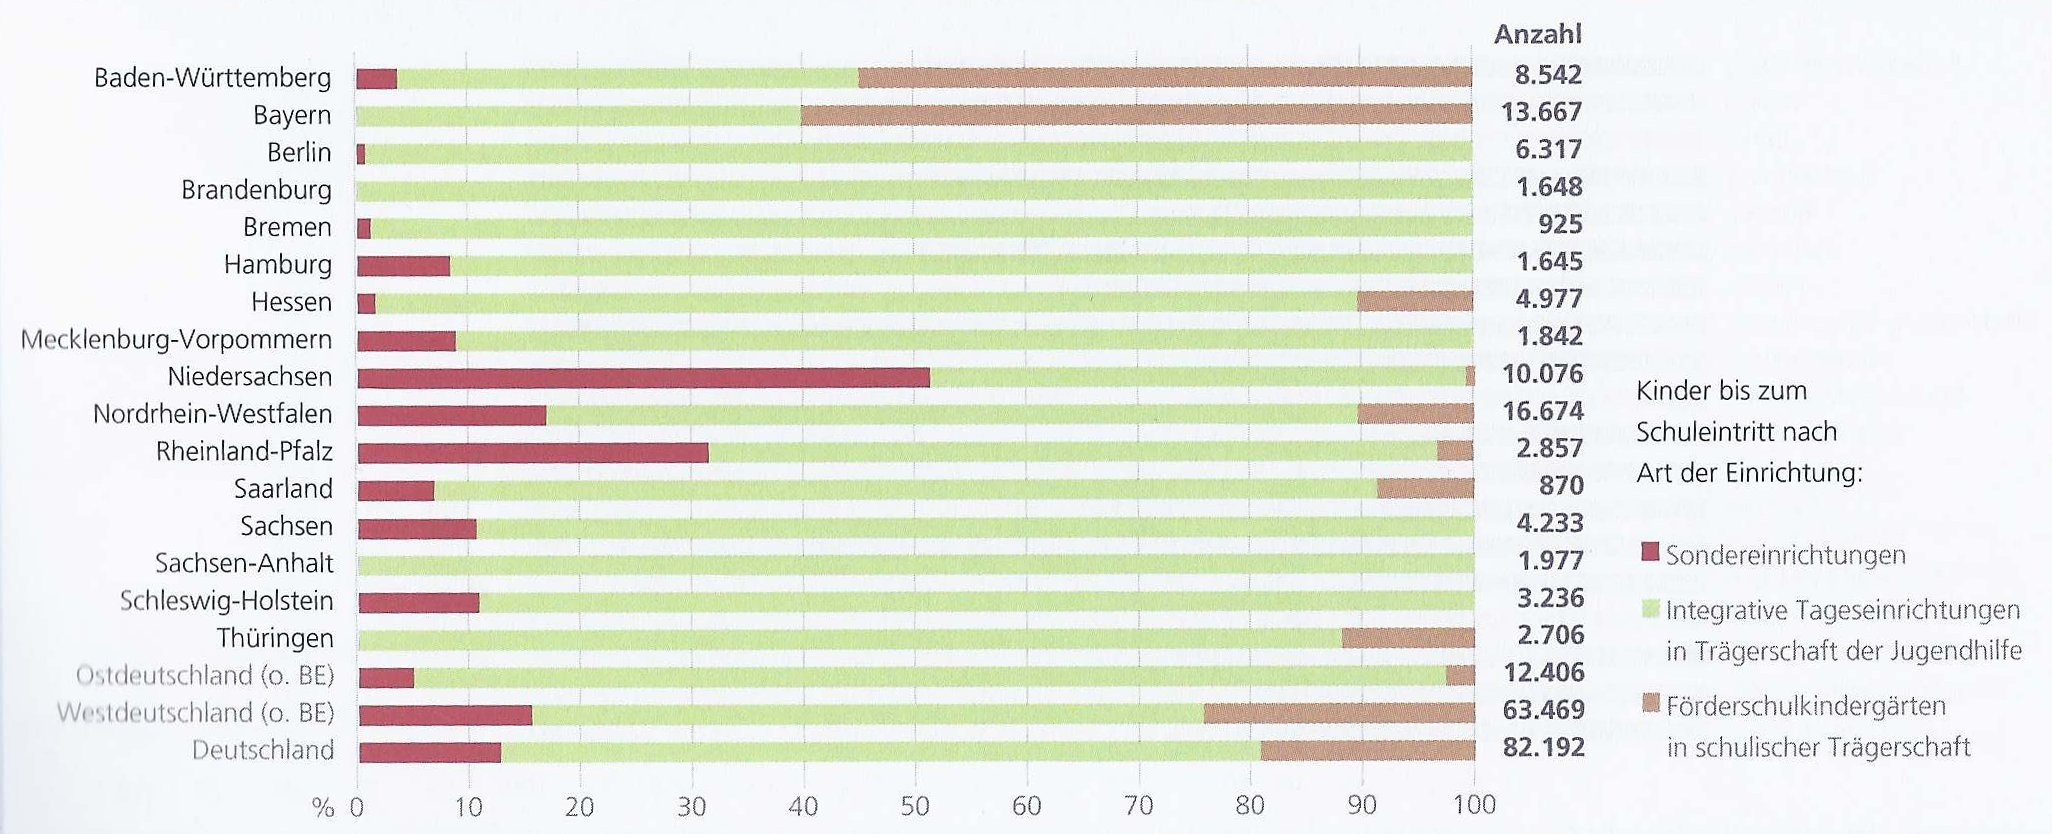
\includegraphics[width=0.95\textwidth]{bilder/bildungsbeteiligung}
  \caption{Bildunsbeteiligung von Kindern mit (drohender) Behinderung nach Art der Einrichtung. Stand: 01.03.2010. In: Bock-Famulla und Lange (2011, 13)}
  \label{bild:bildungsbeteiligung}
\end{figure}


\section{Selbstverständnis des Kindergartens unter Berücksichtigung der Trägervielfalt}\label{sec:kitaSelbst}
Aus den vorangestellten Bezugspunkten und ihren Aufgabenbeschreibungen lässt sich laut Hugoth (2010, 30) das Selbstverständnis des Kindergartens ableiten. Seine Ausdifferenzierungen sollen vorab als Übersicht präsentiert werden:

Der Kindergarten als
\begin{enumerate}
\item erste Stufe des deutschen Bildungssystems,
\item Ergänzung und Unterstützung der Familie,
\item Dienstleister und Teil des Systems der unterstützenden Dienste,
\item Organ des Staates zur Erfüllung seines Wächteramtes und 
\item Ort für alle.
\end{enumerate}

Die inhaltlichen Schwerpunkte der Arbeit im Kindergarten werden nach Hugoth (2010, 19) maßgeblich durch den Träger beeinflusst. Die Einrichtungen weisen ein jeweils trägerspezifisches Profil auf, welches sich in der Auswahl des Personals, in der Organisationsform, im Erscheinungsbild nach außen, in der Schwerpunktsetzung der Arbeit und in der gelebten 'Philosophie' unterscheidet. Dadurch heben sich die Einrichtungen, vor allem die der freien Träger, zum Teil stark voneinander ab. Deutschland hat im Vergleich zu anderen europäischen Ländern die vielfältigste und bunteste Trägerlandschaft. 
Im SGB VIII~§~3 (vgl. Gastiger und Winkler 2009, 312) wird zwischen öffentlichen und freien Trägern unterschieden. Zu den öffentlichen gehören nach §~69 SBG~VIII (ebd., 341) die Landkreise und kreisfreien Städte und die kreisangehörigen Gemeinden. Hugoth (2010, 20) verweist darauf, dass zunehmend mehr Landesgesetze die institutionalisierte Kinderbetreuung in die Hände der Gemeinden vor Ort geben. 

Zu den freien Trägern zählen laut Hugoth: 
\begin{itemize}
\item die kirchlichen Wohlfahrtsverbände Caritas und Diakonie und die katholischen und evangelischen Kirchgemeinden, die mit über 50\,\%
Gesamtanteil (Stand: 2000) das größte Kontingent stellen, 
\item darüber hinaus die Wohlfahrtsverbände wie Arbeiterwohlfahrt, Rotes Kreuz, Paritätischer Wohlfahrtsverband mit ihren Unterorganisationen,
\item Elterninitiativen, Unternehmen und Betriebe sowie
\item gewerbliche Träger\footnote{Auch wenn gewerbliche Träger eigentlich zu den freien Trägern zählen, fallen dem Sprachgebrauch nach alle nicht-staatlichen und nicht-gewerblichen unter die freien Träger.}, zum Beispiel 'Little Giants'. Diese zählen zu den teuren, bilingualen Kindergärten und werden von Weiß (2010) als 'Parallelwelt' für Privilegierte bezeichnet\footnote{Die Homepage gibt weitere Einblicke in das Konzept von Little Giants: http://www.littlegiants.de}.      
\end{itemize}

Die Qualität einer Kindertageseinrichtung hängt nach Hugoth und Jansen (2005, 9 f.) im entscheidenden Maße vom Engagement ihres Trägers ab. Erfolg lässt sich danach bemessen, ob der Träger sein Profil zu schärfen in der Lage ist, indem er es an fachlichen, politischen und gegebenenfalls kirchlichen Anforderungen ausrichtet. Ein professionelles Profil begünstigt eine gute Ausgangsposition im Wettbewerb und dementsprechend berufliche Sicherheit. Die an den Trägerverbund gestellten Anforderungen sind sehr komplex und reichen von der wirtschaftlichen Steuerung und Zukunftssicherung der Einrichtung bis hin zu inhaltlichen Fragen. Dem Träger wie auch der Leitung obliegen eine übergeordnete Steuerungsfunktion. Der Einfluss des Träger auf das Selbstverständnis des Kindergartens kann als entsprechend groß bewertet werden, wenn dieser als „Förderer, Unterstützer und Initiator von Entwicklungen in den Einrichtungen“ (Rückert 2011, 13) verstanden wird. Seine Interessen bilden das übergeordnete Wertesystem der Einrichtung. Wenn sich die kirchlichen Träger, zu denen in der Regel die zahlenmäßig stark vertretenen Gemeinden vor Ort zählen, zu aktuellen sozialpolitischen oder bildungspolitischen Themen öffentlich äußern oder zukunftsweisende Entscheidungen treffen, sind diese nicht nur für einzelne Familien, sondern für die ganze Gesellschaft von nachhaltiger Bedeutung. Somit steht der Träger im Dienste der Gesellschaft. Hier sei als Beispiel die Caritas Kampagne 2011 benannt, in der Inklusion zum Jahresthema ernannt und mit folgendem Leitsatz präsentiert wurde: „Kein Mensch ist perfekt! Behinderte Menschen: Menschen wie du und ich“ (Caritas 2011). Da die Kindergartenträger in eigener Verantwortung ihre Aufgaben beurteilen, hängt die Umsetzung von inklusiver Qualität im Kindergarten laut Rückert (2011, 133) davon ab,  ob die Träger sich ihrer Aufgaben und Verantwortungsbereiche in der gesamtgesellschaftlichen Tragweite bewusst sind und in Abhängigkeit dessen, wo sie in ihren Überlegungen stehen, entsprechende Schritte in Richtung inklusive Erziehungs- und Bildungsarbeit gehen.  
   
\subsection{Der Kindergarten als erste Stufe des deutschen Bildungssystems}
Liegle (2006, 6) schreibt, dass im Zuge der Etablierung des Kindergartens als erste Stufe des deutschen Bildungssystems Fragen in der Öffentlichkeit unterschiedlich diskutiert werden: Ist es die Aufgabe des Kindergartens auf das Lernen in der Schule vorzubereiten oder droht der Kindergarten in Folge dessen zu verschulen? Hugoth (2010, 32) fügt als weiteren Punkt in der Diskussion die Frage nach der Abschaffung der Elternbeiträge an. Die Elternbeiträge werden vom Träger der Einrichtung festgelegt. Befürworter verweisen auf den Schulbesuch, der ebenfalls ohne Beitragszahlung der Eltern auskommt. Kritiker benennen, dass das System Kindergarten dadurch vor allem für freie Träger nicht mehr bezahlbar sei, weil diese den Fehlbetrag aus dem Mangel der Elternbeiträge nicht kompensieren könnten und sich zurückziehen würden. Das birgt die Gefahr, dass die Vielfalt der Träger- und damit der Kindergartenlandschaft geschmälert und die Wahlfreiheit der Eltern gegebenenfalls unterlaufen werden würde. Dass solcherart Fragen öffentlich unterschiedlich diskutiert werden, beweist die Unterschiedlichkeit der Trägerinteressen, stellvertretend für eine pluralistische Gesellschaft. 

Sowohl im SGB VIII als auch im Bildungsplan wird die wechselseitige Zusammenarbeit von Kindergarten und Schule zur Gewährleistung eines guten Übergangs als wichtige Aufgabe formuliert. Nach Liegle (2006,~5~f.) sollen beide Bildungseinrichtungen aufeinander aufbauen, so dass Brüche beim Übergang von der einen zur nächsten Stufe vermieden werden und eine gewisse Kontinuität gewährleistet ist. Er beschreibt jedoch mit kritischem Blick die politische Tendenz in Deutschland, die Misere des Bildungssystems mit Hilfe einer gezielten Förderung auf die Schule beheben zu wollen.
Dass politische Maßnahmen als Folge des PISA-Schocks zu kurz greifen, die den Kindergarten als vorschulische Einrichtung umdeuten wollen, kann mit Hilfe von empirischen Untersuchungen gezeigt werden. Nach  Macon (2002) in Liegle (ebd.) konnte in einer breit angelegten Studie nachgewiesen werden, dass Kinder, die ein stark formalisiertes und strukturiertes Vorschulprogramm besucht hatten, signifikant schlechtere Noten im sechsten Schuljahr bekamen als die Vergleichsgruppe, die Vorschulprogramme mit Betonung auf selbstinitiierten und spielerischen Lernen besucht hatten. 
Laut Becker-Stoll (2009, 46) wird ein Kindergarten zu hinterfragen sein, der den Zusammenhang von Bindung und Bildung missachtet und Lerninhalte statt das Kind und seine Selbsttätigkeit ins Zentrum stellt. Sie argumentiert, dass zu den psychischen Grundbedürfnissen eines Kindes neben Autonomie und Kompetenz auch Bindung gehört. Bindung steht für das Bedürfnis, enge zwischenmenschliche Beziehungen einzugehen und sich innerhalb dieser Interaktion als liebenswert und liebesfähig zu erleben. 
 
Nach Papke (2010) besteht aus der Perspektive der Inklusion die Gefahr, dass manche Bildungsbereiche, die im Bildungsplan benannt werden, nicht für alle Kinder als gleichermaßen wichtig angesehen werden, zum Beispiel Naturwissenschaften und Mathematik. Daran schließt sich die Frage an, gesetzt dem Fall die Fachkräfte in den Einrichtungen sind davon überzeugt, dass alle Kinder in Bezug auf die empfohlenen Bildungsbereiche gleichermaßen anzusprechen sind, was muss bei der Gestaltung dieser Bildungsbereiche berücksichtigt werden, damit diese für alle Kinder interessant und individuell nutzbringend sind? Nur durch eine solche angeregte Auseinandersetzung kann „einem Denken in unterschiedlichen 'Bildungsgruppen' [vorgebeugt werden]“ (Papke 2010).
 
\subsection{Der Kindergarten als Ergänzung der Familie}
Laut Bock-Famulla und Lange (2011, 41) ist die Bildungspartnerschaft zwischen Kindergarten und Eltern von zentraler Bedeutung für die optimale Entwicklung des Kindes im Kindergarten. Jeske (1997, 10) bestätigt ebenfalls, dass, wenn zwischen beiden Lebenswelten positive enge Verbindungen statt starker Gegensätze bestehen, sich dies positiv auf die Entwicklung auswirken würde. Nagel (2009, 204) verweist auf verschiedene Studien, in denen die Interaktionswirkungen zwischen familiärer und außerfamiliärer Betreuung untersucht wird. Die bisherigen Ergebnisse zeigen, dass Entwicklungs- und Bildungschancen vor allem bei ’bildungsfernen’ Familien durch ergänzende Betreuung unterstützt werden können, die Unterstützung jedoch effizienter ist, umso aktiver die Familie selbst unterstützend wirken kann. Der Grund hierfür ist laut Albers (2011, 116) in dem Einfluss der Familie auf die kindliche Entwicklung zu sehen, der als etwa doppelt so hoch gilt wie der Einfluss institutionalisierter Betreuung. Es kann davon ausgegangen werden, dass beide Bereiche sich gegenseitig beeinflussen und eine gute Kooperation und Abstimmung mit den Eltern deshalb betont werden muss. 

Konkrete Vorgaben zur Elternbeteiligung werden laut Schlecht, Förster, Wellner und Mörth (2008, 44) in den Bildungsplänen gemacht. Bereits im Zusammenhang mit der Aufnahme des Kindes wird als wichtig angesehen, dass Eltern die Möglichkeit gegeben wird, gemeinsam mit ihrem Kind in der Gruppe zu hospitieren und in Austausch mit der Erzieherin zu treten, um mit der Einrichtung, ihrem Konzept sowie der Gruppe vertraut zu werden. Zur Aufgabe der Erzieherin gehört es familiäre, kulturelle und religiöse Besonderheiten des Kindes zu berücksichtigen und diese in den Alltag einzubeziehen. 'Bildungspartnerschaft' mit den Eltern kann durch regelmäßige Elternabende, jährliche Entwicklungsgespräche und allgemeinen Austausch über die Aktivitäten des Kindes erfolgen. Wünschenswert ist auch, dass die Eltern die Möglichkeit bekommen, ihre Interessen in die pädagogische Arbeit einzubringen und bei Planungs\- und Entscheidungsprozessen berücksichtigt werden.

\subsection{Der Kindergarten als Dienstleister}
Nach Hugoth (2010, 34 f.) hat sich in den letzten Jahren bedingt durch eine kritischere Erwartungshaltung von Seiten der Eltern, des Trägers aber auch der Behörden im Bereich der Kinder- und Jugendhilfe der Kindergarten zu einem Dienstleister entwickelt. An selbigen werden  Fragen gerichtet, ob er in Anbetracht dessen, was er leistet, das wert ist, was in ihn investiert wird und ob die erbrachten Leistungen den Bedürfnissen der Kinder und Familien entsprechen. Zudem verstehen sich Eltern nicht mehr als 'Laien', die ihre Kinder von 'Profis' betreuen lassen, sondern vielmehr als Kunden, die ausgewiesene Dienstleistungen erwarten und wird ihren Erwartungen nicht entsprochen, sich nach anderen Kindergartenplätzen umschauen. Er (2010, 35) verweist auf den Aspekt, dass in vielen Kommunen ein Konkurrenzdruck durch ein Überangebot an Kindergartenplätzen und eine schwindende Kinderzahl entsteht. Das zwingt die Einrichtung ihre Qualität unter Beweis zu stellen, um konkurrenzfähig zu bleiben. 
Kritisch merkt er (2010, 36 f.) jedoch an, dass eine Einrichtung, die in Leistungskategorien denkt und stets die Bedarfe des Kunden, also der Eltern, im Blick hat, an ihre Grenzen stoßen wird, da sie auch gesetzlichen Vorgaben, dem vom Träger vorgegebenen Profil, fachlichem Wissen sowie beruflicher Erfahrung verpflichtet ist. Hierbei können Elterninteressen und eigene Vorstellungen, was das 'Beste' für das Kind ist kollidieren. Fritz und Hugoth (2010, 28 f.) empfehlen deshalb von einer „Dienstleistungsorientierung“ statt einem „Dienstleistungsunternehmen“ zu sprechen. Eine reine Orientierung an Kundenzufriedenheit, wie es von wirtschaftlichen Unternehmen bekannt ist, ist der Qualität der Einrichtung nicht förderlich. 

\subsection{Der Kindergarten als Organ des Staates zur Erfüllung des Wächteramtes}
Die Aufgabe des Wächteramtes ist gesetzlich klar geregelt. Der Träger ist in der Pflicht diesen Auftrag zu erfüllen, Spielraum bei der Umsetzung gibt es in diesem Fall nicht.
 
Hugoth (2010, 32) verweist darauf, dass, um die Kooperation und Vernetzung der Hilfesysteme zu verbessern, die Kindertagesstätten in das staatliche Wächteramt einbezogen wurden, welches nun zu ihrem Betreuungsauftrag gehört. Laut ihm (2010, 33) kann die Umsetzung eines so definierten Betreuungsauftrag zu einem Interrollenkonflikt der Erzieherin führen. Die unterschiedlichen Rollen, in denen sie sich befindet, einerseits Wächter und Anwalt des Kindes, andererseits Partner der Eltern, können im Einzelfall zuwider laufen. Transparenz des Kindergartens gegenüber den Eltern sei deshalb geboten, das heißt konkrete Interessen, Inhalte, Arbeitsweisen und normative Grundlagen des Kindergartens sollten klar definiert und mit den Eltern kommuniziert werden.

\subsection{Der Kindergarten als Ort für alle}\label{OrtFuerAlle}
Statistiken zeigen, dass nahezu jedes Kind in Deutschland einen Kindergartenplatz in Anspruch nimmt, weshalb laut Kron (2010, 32 f.) davon ausgegangen werden kann, dass die Heterogenität\footnote{Nach Prengel und Heinze (2012) bedeutet 'heterogen' verschieden, anders, plural. Heterogenität stellt ein Verhältnis von Verschiedenen dar, die einander nicht untergeordnet, sondern gleichgestellt sind. Im vorliegenden Kontext bezieht sich der Begriff auf die zu respektierenden Differenzen zwischen einzelnen Kindern, also auf ihre individuelle Einzigartigkeit innerhalb der Gruppe.}
der Kindergartengruppe die gesellschaftliche Vielfalt repräsentiert, davon ausgenommen jedoch die Zahl der in Sondereinrichtungen betreuten Kinder. Die europäische multikulturelle Gesellschaft zeichnet sich durch immer komplexer werdende Differenzen und eine wachsende gesellschaftliche Vielfalt aus, in der traditionelle Unterscheidungsmerkmale verschwimmen. Gründe hierfür sieht Speck-Hamdan (2011, 16) in der Migrationsbewegung und in Individualisierungsprozessen. Der Kindergarten wird somit zum Spiegel dieser Vielfalt – „die Welt trifft sich im Kindergarten“\footnote{Buchtitel von Oberhuemer, Soltendieck und Ulrich, 2001}.
 
Um das Spektrum an Unterschieden überschaubar zu machen, werden eine Reihe von Kategorien angelegt. Im derzeitigen Interesse der Sozialwissenschaften liegen laut Albers (2011, 37) vor allem die Kategorien Migration, Behinderung, sozialer Hintergrund und Geschlechtszugehörigkeit.
Wenn jedoch nur ein Unterscheidungsmerkmal untersucht wird, merkt 
Speck-Hamdan (2011, 16) kritisch an, dass es zu Verkürzungen kommen kann, weil sich Differenzlinien überschneiden und die Individualität eines Menschen gerade dadurch bestimmt wird, dass der Mensch mit mehreren Facetten zu beschreiben ist. Deshalb sind die in den Sozialwissenschaften in den Vordergrund gestellten Facetten bei weitem nicht alle, anhand derer Kinder voneinander unterschieden werden können. Mögliche weitere Kategorien zur Wahrnehmung pluraler Differenzen in einer Kindergartengruppe bestehen hinsichtlich Alter, ethnisch-kultureller Herkunft, Sprache, Glaubensrichtung, Eltern, Geschwister, Familienkultur und Sozialisation, Qualität ihrer Bindungserfahrungen, Bildungsbiografie, Lernumfeld, ökonomischer Lebenslage, Entwicklungsverlauf sowie bisheriger Erfahrungen in gleichaltrigen Gruppen. 

Eine Bestandsaufnahme hinsichtlich der Merkmale Migrationshintergrund, soziale Benachteiligung und Entwicklungserschwernisse schließt sich an, die Antwort auf die Frage geben soll, wer im Kindergarten aufeinander trifft. 

Laut Roth und Terhart (2009, 8) hat im Jahre 2008 etwa jedes vierte Kindergartenkind einen Migrationshintergrund, das heißt, es selbst oder mindestens eines seiner Elternteile oder auch eines seiner Großelternteile ist seit der Nachkriegszeit in Deutschland eingewandert. Hierbei wird ein großer Ost-West-Unterschied deutlich. In den westdeutschen Bundesländern haben 29\,\% der über Dreijährigen einen Migrationshintergrund, in den ostdeutschen Bundesländern lediglich 6\,\%. Von allen Migrantenkindern besucht nahezu jedes dritte Kind eine Gruppe, die sich wiederum zu mindestens 50\,\% aus Kindern mit Migrationshintergrund zusammensetzt. Bei Kindern mit Migrationshintergrund handelt es sich ebenfalls um eine sehr heterogene Gruppe, über die nur sehr schwer allgemeine Aussagen getroffen werden können. Ein verbindender Aspekt ist die häufige Zwei- oder Mehrsprachigkeit. Unterschiede machen sich fest an den Herkunftsländern, der ethnischen Zugehörigkeit, der Aufenthaltsdauer, dem rechtlichen Status und den Beweggründen der Eltern nach Deutschland zu kommen. Der kulturelle Hintergrund kann nach Albers (2011, 38) nicht ohne Bezugnahme auf Faktoren, wie Geschlecht, sozialer Status, Einkommen, Bildungshintergrund, Religion und Alter gesehen werden.
 
Was sagt ein Migrationshintergrund über das Kind aus? Laut Roth und Terhart (2009, 77~f.) steht der Migrationshintergrund in Korrelation zu Armutsverhältnissen. 
Mittels der Längsschnittstudie zur Kinderarmut in Deutschland vom Institut für Sozialarbeit und Sozialpädagogik (1997 - 2005) wurde herausgefunden, dass bei der Gruppe der Vorschulkinder die Armutsquote bei Kindern mit Migrationshintergrund mit über 40\,\% mehr als doppelt so hoch ist wie bei den Kindern mit deutschem Pass. Gründe für Einkommensarmut der Familien sind vor allem in Zugangsbarrieren zum Ausbildungs- und Arbeitsmarkt und einem häufig niedrigeren Bildungsniveau der Eltern zu suchen. 
Laut Weiß (2010) wächst auf der einen Seite der Wohlstand, zwei Drittel der Kinder in Deutschland geht es materiell so gut wie keiner Generation vorher, auf der anderen Seite wächst die Gruppe der sozial Ausgegrenzten, 2~bis~2,5 Millionen Kinder und Jugendliche leben bis zum 18. Lebensjahr von staatlicher Unterstützung. 
Forschungen haben ergeben, dass Armut an sich noch kein direktes Risiko für die kindliche Entwicklung darstellt, jedoch die Wahrscheinlichkeit für Entwicklungsgefährdungen, bedingt durch komplexe Unterversorgung oder ein unzureichendes oder schädigendes Erziehungsverhalten seitens der Bezugspersonen, erhöht ist. 
Nach Weiß (2000, 52 f.) hängt das Entwicklungsrisiko vom Ausmaß der Armut, sowohl von ihrer Dauer als auch von ihrer Komplexität und Intensität, und zudem von den Bewältigungsstrategien der betroffenen Familien ab. Bei chronischer Armut besteht ein wesentlich größeres Risiko als bei kürzeren Armutsperioden, da individuelle Handlungsspielräume in zentralen Lebensbereichen eingeengt werden oder verloren gehen.
Vor allem bei chronischer Armut werden laut ihm die betroffenen Menschen nicht selten von der Erwerbsgesellschaft ausgegrenzt und fühlen sich in Folge dessen überflüssig, nutzlos und nicht gebraucht, wodurch Zukunftsperspektiven schwinden und gehäuft Selbstentwertung und Verunsicherung auftreten. Wenn Kinder in eine solche familiäre Situation hinein geboren werden, dann ist das Risiko erhöht, dass sie auf Eltern treffen, die nicht die Kraft haben den Aufgaben der Pflege und Erziehung hinreichend nachzukommen und die intuitive und empathische Kompetenzen vermissen lassen, da sie bedrängt von hoher existenzieller Unsicherheit in ihren Alltagsproblemen gefangen sind.   
Grundsätzlich besteht „ein plausibler und auch empirisch nachgewiesener Zusammenhang zwischen soziökonomischen und psychosozialen Belastungssituationen sowie der kindlichen Entwicklungsgefährdung bis hin zu manifesten Behinderungen“ (Weiß 2000, 51).

Biedinger (2009, 197) hat die Folgen von Einkommensarmut auf die kognitive Entwicklung, das Sozialverhalten und den Wortschatzumfang von 3 bis 4-jährigen Kindern untersucht. Die Ergebnisse zeigen, dass der Einfluss der Armut auf die kindliche Entwicklung und den Wortschatz, jedoch nicht auf das Sozialverhalten signifikant ist und selbst unter Kontrolle der Bildung der Bezugsperson bestehen bleibt. Es konnte gezeigt werden, dass der häusliche Lern- und Erfahrungsspielraum entscheidenden Einfluss auf die Entwicklung nimmt und bei Familien in Armut als ebenfalls verarmt betrachtet werden kann, genauso wie ihre Entfaltungs- und Bildungsmöglichkeiten und die Förderung ihrer individuellen Neigungen und Fähigkeiten.

Kinder in Armut sind eine Herausforderung für inklusive Erziehungs- und Bildungsarbeit, weil sie einerseits in ihrer Verschiedenheit zu anderen gesehen anerkannt werden müssen, aber bloße Anerkennung keine Antwort auf eine „wachsende gesellschaftliche Ungleichheit und ihre Exklusion fördernden Folgen“ (Weiß 2010) ist. Inklusion verfolgt das Ziel sozialer Gerechtigkeit, das heißt, dass dem Bildungssystem eine kompensatorische Funktion zukommt.       
 
Da Behinderung nach Albers (2011, 38) aus der Wechselwirkung von funktionaler Beeinträchtigung im Zusammenwirken mit sozialen Faktoren entsteht, ist auch hier ein mehrdimensionaler Blick erforderlich. Kinder mit Behinderung sind im Kindergarten zunächst einmal Kinder mit bestimmten Voraussetzungen, zum Beispiel Hörverlust, Sehbeeinträchtigung oder Down-Syndrom, die sich erschwerend auf ihre Entwicklung und ihr Lernen auswirken. Jeder Diagnose liegt eine Spannweite von leichter bis schwerer Ausprägung zugrunde. Kinder mit Down-Syndrom zum Beispiel haben eine Intelligenzminderung und trotzdem gibt es Kinder unter ihnen, die das Abitur absolvieren und wiederum andere, die kaum beschulbar sind. Zudem können auch mehrere dieser bestimmten Voraussetzungen bei einem Kind vorliegen, was die Gruppe der Kinder mit Behinderung insgesamt zu einer sehr heterogenen Gruppe macht. Sarimski (2012, 10) gibt die Prävalenz für unterschiedliche Formen von Behinderung mit insgesamt drei bis vier Prozent an. Darunter zählt er Kinder mit einer Seh- oder Hörschädigung, Körperbehinderung, Spracherwerbsstörung, Lern- oder geistigen Behinderung oder mit Autismusspektrumsstörung. 
Eine sehr viel größere Gruppe bilden Kinder mit Entwicklungsrückständen ohne erkennbare biologische Beeinträchtigung, Teilleistungsstörungen, Verhaltensauffälligkeiten oder in außergewöhnlichen Belastungssituationen, zum Beispiel Kinder psychisch kranker oder suchtkranker Eltern. Nach Klein (2010, 12) zeigt insgesamt jedes fünfte Kind eine solche Entwicklungsproblematik. 

Zusammenfassend kann nach Kron (2010, 32 f.) festgehalten werden, dass Kinder in Deutschland unter sehr unterschiedlichen Bedingungen aufwachsen, so dass Heterogenität eine soziale Tatsache ist. 
Gemeinsam ist allen Kindern, dass sie Kinder sind und dass sie alle einzigartige Bedürfnisse haben. 
Da die Unterschiedlichkeit der Kinder als reale Ausgangslage anerkannt werden muss, gilt es laut Sarimski (2012, 11) pädagogische Lösungen zu entwickeln, die dieser Vielfalt gerecht werden. Das fokussierte Ziel muss demzufolge lauten, ausnahmslos alle Kinder in gleichermaßen guter Qualität betreuen, erziehen und bilden zu wollen.  

\section{Qualitätsmanagement in Kindertageseinrichtungen}

Laut Esch, Klaudy, Micheel und Stöbe-Blossey (2006, 9) ging die Bildungsdebatte Anfang der 90er Jahre Hand in Hand mit der nationalen und internationalen Diskussion über Qualitätsfragen im Elementarbereich, verbunden mit erhöhten Erwartungen an den Kindergarten, was dieser zu leisten habe und wie dieser beschaffen sein sollte. Wie bereits erwähnt sind die Träger der Kindertagesstätten seit der Erneuerung und Erweiterung des Kinder- und Jugendhilfegesetzes (§§ 22 bis 24a SBG VIII) zur Qualitätsentwicklung verpflichtet. Eine steigende Qualität soll unter anderem Antwort auf bildungs- und sozialpolitische Herausforderungen geben, wie den erhöhten Anteil an Kindern mit Migrationshintergrund in Kindergartengruppen.
Bemühungen, Qualitätsmerkmale festzulegen und qualitätssichernde Maßnahmen zu etablieren, erfolgten laut Hugoth (2010, 30 f.) zum Beispiel durch die Implementierung der Bildungspläne oder die 1999 vom Bundesministerium für Familie, Frauen, Senioren und Jugend ins Leben gerufene Nationale Qualitätsinitiative im System der Tageseinrichtungen für Kinder (NQI). Die aktuellste Antwort auf die Qualitätsfrage ist die Nationale Untersuchung zur Bildung, Betreuung und Erziehung in der frühen Kindheit (NUBBEK), erste Ergebnisse liegen seit 2012 vor. Durch die gemeinsame Anstrengung von Tietze, Becker-Stoll, Bensel, Eckhardt, Haug-Schnabel, Kalicki, Keller und Leyendecker (2012, 4) hat sich die  NUBBEK-Studie zum Ziel gesetzt auf hinreichend großer Datenbasis die Qualität in unserem Früherziehungssystem sowohl bezogen auf die Betreuungsqualität in der Familie als auch im institutionellen Setting zu untersuchen. 
  
\subsection{Pädagogische Qualität und ihre Dimensionen}

Tietze (2004, 406) definiert den Qualitätsbegriffs sehr allgemein: Mit Qualität wird die Beschaffenheit einer Dienstleistung bezeichnet und durch eine Reihe charakteristischer und überprüfbarer Eigenschaften näher beschrieben, welche für den Nutzer der Dienstleistung von Bedeutung sind. In dieser Begriffsbestimmung können in Bezug auf das Untersuchungsfeld Kindergarten drei Variablen näher bestimmt werden:

\begin{enumerate}
\item Die Dienstleistung als eine pädagogische bezieht sich auf die Trias Betreuung, Bildung und Erziehung.
\item Genutzt wird diese Dienstleistung von den Eltern, den Kindern und den Erzieherinnen.
\item Die Dimensionierung der Eigenschaften in Strukur-, Orientierungs- und Prozessqualität wird laut  Tietze (2004, 407) als hilfreich erachtet. Zudem kann laut Behr (2009, 67) die Ergebnisqualität als weiteres Unterscheidungskonstrukt festgelegt werden.
\end{enumerate}

Laut Ahnert (2011, 153 f.) stellt das Messen von Qualität institutionalisierter Betreuung ein schwieriges Unterfangen dar, da von Seiten der betroffenen Nutzer unterschiedliche Qualitätsvorstellungen zu erwarten sind beziehungsweise die Nutzer dieselben Eigenschaften möglicherweise unterschiedlich bewerten. Aus Elternsicht würde sich die Qualität der Einrichtung beispielsweise an Wohnortnähe und adäquaten Betreuungszeiten -- Merkmale, die mit ihrem Beruf gut vereinbar sind -- bemessen. Das Qualitätsmerkmal 'verlängerte Öffnungszeiten' würde aber aus der Perspektive der Erzieherin bedeuten, einen Arbeitsplatz mit Schichtbetrieb und daraus resultierend familienunfreundliche Arbeitszeiten vorzufinden.  
Um Klarheit in die Qualitätsdebatte zu bringen, wurde von der National Association for Education of Young Children (NAEYC) schon vor längerer Zeit das Kind ins Zentrum der Debatte gestellt. Somit gilt, wenn nach Tietze (2004, 407) von pädagogischer Qualität gesprochen wird, dann wird ein konkreter Bezug zur kindlichen Entwicklung vorausgesetzt. Pädagogische Qualität ist nur dann gegeben, „wenn diese das körperliche, emotionale, soziale, intellektuelle Wohl sowie die gegenwärtigen und zukünftigen Entwicklungen der Kinder in diesen Bereichen fördert und die Familien in ihrer Betreuungs- und Erziehungsaufgabe unterstützt“ (Tietze 2004, 407). Um pädagogische Qualität zu bestimmen, müssen vorab Qualitätsindikatoren in Bezug auf einen guten Kindergarten unter Perspektive des Kindes und seiner Entwicklungsförderung entwickelt werden. Die Qualität als Ergebnis misst sich dann daran, inwieweit diese Festlegungen in der Praxis der Einrichtung umgesetzt werden konnten. 

Kritisch merken Honig et al. (2004, 13 f.) an, dass die dominierende frühpädagogische Qualitätsdebatte, die wie selbstverständlich auf das Kind und seine Entwicklung sowie auf den Handlungsraum der einzelnen Einrichtung bezogen ist, eine Verengung darstellt, weil wichtige Aspekte unberücksichtigt bleiben. Kindergärten sind 'soziale Räume' und als solche in komplexe gesellschaftliche Funktionszusammenhänge und kulturelle Kontexte eingebettet. „Daher sind die Maßstäbe für einen guten Kindergarten nicht nur vielfältig, sondern unvermeidlich strittig; bei genauem Hinsehen weisen sie sogar eine dilemmatische Struktur auf, weil das System der Tageseinrichtungen für Kinder in ein Netz heterogener generalisierter Erwartungshorizonte eingebunden ist. Kindergärten sind entsprechend Schauplatz von Auseinandersetzungen um unterschiedliche Interessen, die mit ungleichen Einflusschancen ausgestattet sind. [...] Kindergärten vermögen ihre Güte also nicht autonom zu bestimmen“, sondern müssen die Differenzen immer wieder austarieren. 
Nach Meinung der Autoren sollte der Qualitätsdiskurs von der Frage bestimmt werden, wie sich die unterschiedlichen Erwartungen miteinander vereinbaren lassen.

Die Weiterentwicklung der pädagogischen Arbeit und die Qualitätssicherung ist laut Tietze, Dittrich, Grenner, Groot-Wilken, Sommerfeld und Viernickel (2004, 16 f.) in der Regel Aufgabe der Leitung. Davon abweichend können Qualitätsbeauftragte als Koordinatoren vom Träger gestellt werden oder aber die Leitung überträgt diese Aufgabe einer Fachkraft aus dem Team. 
Der Gewinn in der Anwendung von Qualitätsmanagementverfahren für die pädagogische Fachkraft liegt nach Volkert (2008, 75) in einem  wachsenden professionellen Selbstverständnis, das entsteht, wenn Prozesse, um sie zu verbessern, differenziert und reflektiert betrachten werden.

Nach Behr (2009, 14) impliziert pädagogische Qualität im Bezug auf Kinder mit besonderen Bedürfnissen stets die Dimension der Inklusion, da durch die Behinderung zugleich die Aufgabe der Einbeziehung und Partizipation gestellt ist. 

In den folgenden Kapiteln werden die vier Qualitätsdimensionen vorgestellt und durch Beispiele bestehender Qualitätsstandards vor allem im Hinblick auf Inklusion ergänzt.

\subsection{Strukturqualität}
\label{subsec:Strukturquali}
Laut Tietze (2004, 407) werden unter Strukturqualität Aspekte zusammengefasst, die situationsunabhängig, zeitlich stabil und politisch regulierbar sind. Solche strukturellen Rahmenbedingungen können wiederum unterschieden werden in einerseits der Einrichtung zur Verfügung stehende materielle Ressourcen und andererseits personelle Ressourcen. Unter materiellen Ressourcen werden die vorhandenen Räume und deren Ausstattung, die Finanzierung des Personals, der Betreuungsschlüssel, die Gruppengröße und die Gruppen- und Personalstruktur sowie die vorgesehenen Zeiten für mittelbare pädagogische Arbeit\footnote{ Mittelbare pädagogische Arbeit umfasst alle Aufgaben, die zusätzlich zu der direkten Arbeit mit den Kindern bestehen, zum Beispiel Elternarbeit, regelmäßige Dokumentation über Bildungs- und Entwicklungsförderung der Kinder oder Qualitätsentwicklung.} zusammengefasst, unter personelle Ressourcen zählt die Qualifikation der Fachkräfte, festgelegt durch Curriculum und Standards in der Erzieherinnen-Ausbildung. 

Nach Viernickel und Schwarz (2009, 15) werden die Ausbildung, Qualifikation und Bezahlung der pädagogischen Fachkräfte sowie der Betreuungsschlüsse und die Gruppengröße als zentrale strukturelle Rahmengrößen eingestuft, weil bei ihnen ein bedeutsamer Zusammenhang zur kindlichen Entwicklung und zu Aspekten der Prozessqualität nachgewiesen werden konnte. 
Hierfür ist der Betreuungsschlüssel ein geeignetes Beispiel. Die Expertise von Viernickel und Schwarz zur Bestimmung des Betreuungsschlüssels zeigt, je günstiger die Fachkraft-Kind-Relation ausfällt, desto positiver gestaltet sich die Prozessqualität, das heißt die pädagogischen Interaktionen, die bildungsanregenden Impulse, das Wohlbefinden und letztlich die Entwicklung der Kinder. Der Schwellenwert für drei bis sechsjährige, bei dessen Unterschreitung das Wohlbefinden der Kinder gefährdet ist, liegt bei circa eine Fachkraft auf acht Kinder. Die Ergebnisse dieser Expertise zeigen, dass die notwendigen Standards bei der Mehrzahl der Bundesländer nicht erreicht werden, weshalb die Bildungsansprüche, die in den Bildungsplänen benannt werden, schwer umzusetzen sind.

Qualitätsstandards in Bezug auf Kinder mit besonderen Bedürfnissen können laut Sarimski (2012, 145~f.) durch die Elternbefragung von Kobelt Neuhaus (2001) und die Befragung der pädagogischen Fachkräfte durch Dichans (1990) gewonnen werden:
 
\begin{itemize}
\item Aus Elternsicht: Gruppenstärke von nicht mehr als 18 Kindern, davon höchstens ein bis zwei Kinder mit Behinderung und zwei Fachkräfte 
beziehungsweise 
aus der Sicht der Erzieherinnen: Gruppenstärke von maximal 15 Kindern bei nicht mehr als einem Drittel Kindern mit Behinderung und drei Mitarbeitern, davon mindestens zwei Fachkräfte
\item barrierefreie Zugangsmöglichkeiten und entsprechende Ausstattung mit Materialien, die auf die spezifischen Bedürfnisse der Kinder zugeschnittenen sind
\item ausreichend Zeit, in der die Erzieherinnen von der Betreuung der Kinder freigestellt sind, um sich mit heilpädagogischen Fragen innerhalb und außerhalb des Teams zu befassen, Angebote sowie spezielle Fördermaßnahmen differenziert zu planen und intensive Beratung durch Fachdienste wahrzunehmen
\item Fortbildungsmöglichkeiten
\end{itemize}

\subsection{Orientierungsqualität}
Nach Tietze (2004, 411) erfordert ein entwicklungsfördernder Umgang mit dem Kind hohe formale und berufsbezogene Qualifikation. Eng im Zusammenhang mit der Ausbildungsqualität der Erzieherinnen steht die Orientierungsqualität. Diese umfasst laut ihm (2004, 407 f.) pädagogische Vorstellungen, Werte und Überzeugungen der Erzieherin. Welches Bild sie vom Kind, aber auch von den Eltern hat, wird ihre pädagogische Arbeit maßgeblich bestimmen. Für gelingende inklusive Bildungsprozesse ist eine ressourcenorientierte Haltung als Grundvoraussetzung anzusehen. Haltungen und Orientierungen werden in der Ausbildung erworben und in Fortbildungen vertieft, sind aber auch von der Persönlichkeit abhängig. 
Da die Empathiefähigkeit der Erzieherin Voraussetzung für eine sichere Bindungsbeziehung zum Kind ist, sehen Haderlein und Sell (2007, 24) die Notwendigkeit, die Frage nach der Persönlichkeit offen zu stellen. Denn, „nicht jeder Mensch ist in der Lage im Prozess der Praxis der Betreuung, Erziehung und Bildung von Kindern aus seiner Person selbst heraus eine hohe Qualität zu entfalten, auch und nicht selten trotz eines hohen Reflexionsgrades auf theoretischem Niveau“ (Haderlein und Sell 2007, 24). Anders als die Merkmale der Strukturqualität sind die Rahmengrößen der Orientierungsqualität nicht direkt politisch steuerbar, werden jedoch ebenso als zeitlich stabil angesehen. Oft werden übergeordnete Werte auch vom Träger vorgegeben. Sie werden aber auch von den Mitarbeiterinnen erarbeitet und der Konzeption der Einrichtung unter Beachtung vorhandener Rahmenrichtlinien zugrunde gelegt, so dass eine Verständigungsgrundlage nach innen und außen geschaffen wird. 

\subsection{Prozessqualität}\label{Prozessqualität}
Zur Prozessqualität zählt „all das, was den konkreten Erfahrungs- und Erlebnisraum des Kindes in der Einrichtung unmittelbar gestaltet und beeinflusst“ (Tietze 2001, 7). Prozessqualität bezieht sich auf den Kindergartenalltag mit seinen Interaktionen und Erfahrungen, die das Kind innerhalb seiner sozialen und räumlichen Umwelt macht. Die Prozessqualität wird als dynamisches Konstrukt bezeichnet, da sie situationsabhängig ist. Die Ergebnisse der NUBBEK-Studie herausgegeben von Tietze et al. (2012, 8) weisen im Bereich der Prozessqualität erhöhte Werte auf, wenn keine Altersmischung vorliegt und wenn offene, das heißt gruppenübergreifende Arbeit stattfindet. Es zeigen sich niedrigere Werte, je höher der Anteil an Kindern mit Migrationshintergrund ist. Weiterhin zeigt sich, dass die Prozessqualität entscheidend von den Persönlichkeitsmerkmalen der Erzieherin bestimmt wird, insbesondere ihrer Zufriedenheit. Hierin drückt sich die Abhängigkeit der Prozessqualität von Rahmenbedingungen der Struktur- und Orientierungsqualität aus.   

\subsection{Ergebnisqualität}
Die Ergebnisqualität ist vor allem für die Inklusionsperspektive relevant. Nach Behr (2009, 67) werden unter Ergebnisqualität  wahrnehmbare beziehungsweise messbare Auswirkungen einer Maßnahme verstanden, so dass gezeigt werden kann, ob durch spezifische Maßnahmen Entwicklungsfortschritte bei Kindern mit Entwicklungsgefährdungen erreicht werden können. Für die Beantwortung dieser Fragen können entwicklungsdiagnostische Testverfahren eingesetzt werden.


